%%
%% This is file `sample-authordraft.tex',
%% generated with the docstrip utility.
%%
%% The original source files were:
%%
%% samples.dtx  (with options: `authordraft')
%% 
%% IMPORTANT NOTICE:
%% 
%% For the copyright see the source file.
%% 
%% Any modified versions of this file must be renamed
%% with new filenames distinct from sample-authordraft.tex.
%% 
%% For distribution of the original source see the terms
%% for copying and modification in the file samples.dtx.
%% 
%% This generated file may be distributed as long as the
%% original source files, as listed above, are part of the
%% same distribution. (The sources need not necessarily be
%% in the same archive or directory.)
%%
%% The first command in your LaTeX source must be the \documentclass command.
\documentclass[sigconf,authordraft]{acmart}
\graphicspath{{figures/}}
\usepackage[ruled,vlined,linesnumbered]{algorithm2e}
\usepackage{graphicx}
\usepackage{subcaption}
%% NOTE that a single column version may be required for 
%% submission and peer review. This can be done by changing
%% the \doucmentclass[...]{acmart} in this template to 
%% \documentclass[manuscript,screen,review]{acmart}
%% 
%% To ensure 100% compatibility, please check the white list of
%% approved LaTeX packages to be used with the Master Article Template at
%% https://www.acm.org/publications/taps/whitelist-of-latex-packages 
%% before creating your document. The white list page provides 
%% information on how to submit additional LaTeX packages for 
%% review and adoption.
%% Fonts used in the template cannot be substituted; margin 
%% adjustments are not allowed.
%%
%% \BibTeX command to typeset BibTeX logo in the docs
\AtBeginDocument{%
  \providecommand\BibTeX{{%
    \normalfont B\kern-0.5em{\scshape i\kern-0.25em b}\kern-0.8em\TeX}}}

%% Rights management information.  This information is sent to you
%% when you complete the rights form.  These commands have SAMPLE
%% values in them; it is your responsibility as an author to replace
%% the commands and values with those provided to you when you
%% complete the rights form.

% \setcopyright{acmcopyright}
% \copyrightyear{2018}
% \acmYear{2018}
% \acmDOI{10.1145/1122445.1122456}

%% These commands are for a PROCEEDINGS abstract or paper.

% \acmConference[Woodstock '18]{Woodstock '18: ACM Symposium on Neural
%   Gaze Detection}{June 03--05, 2018}{Woodstock, NY}
% \acmBooktitle{Woodstock '18: ACM Symposium on Neural Gaze Detection,
%   June 03--05, 2018, Woodstock, NY}
% \acmPrice{15.00}
% \acmISBN{978-1-4503-XXXX-X/18/06}


%%
%% Submission ID.
%% Use this when submitting an article to a sponsored event. You'll
%% receive a unique submission ID from the organizers
%% of the event, and this ID should be used as the parameter to this command.
%%\acmSubmissionID{123-A56-BU3}

%%
%% The majority of ACM publications use numbered citations and
%% references.  The command \citestyle{authoryear} switches to the
%% "author year" style.
%%
%% If you are preparing content for an event
%% sponsored by ACM SIGGRAPH, you must use the "author year" style of
%% citations and references.
%% Uncommenting
%% the next command will enable that style.
%%\citestyle{acmauthoryear}

%%
%% end of the preamble, start of the body of the document source.
\newcommand{\wl}[1]{\textcolor{red}{#1}}
\begin{document}

%%
%% The "title" command has an optional parameter,
%% allowing the author to define a "short title" to be used in page headers.
\title{A Framework of Multi-stage Dynamic Pricing for Meal-Delivery Platform}

%%
%% The "author" command and its associated commands are used to define
%% the authors and their affiliations.
%% Of note is the shared affiliation of the first two authors, and the
%% "authornote" and "authornotemark" commands
%% used to denote shared contribution to the research.
\author{Zhuolin Wu}
\authornote{Both authors contributed equally to this research.}
\email{wuzhuolin@meituan.com}
\author{Li Wang}
\authornotemark[1]
\email{mxdsjyd@163.com}
\affiliation{%
  \institution{Meituan-Dianping Group}
  \city{Beijing}
  \country{China}
}
\author{xxx,xxx}

\email{xxx@meituan.com}

\affiliation{%
  \institution{Meituan-Dianping Group}
  \city{Beijing}
  \country{China}
}

%%
%% By default, the full list of authors will be used in the page
%% headers. Often, this list is too long, and will overlap
%% other information printed in the page headers. This command allows
%% the author to define a more concise list
%% of authors' names for this purpose.
\renewcommand{\shortauthors}{Zhuolin and Li, et al.}

%%
%% The abstract is a short summary of the work to be presented in the
%% article.
\begin{abstract}
 The restaurant meal-delivery is going through an explosive growth as this service becomes more and more fashionable. The aim of the meal-delivery platform is to provide effective and efficient service at lower delivery cost. In this paper, we propose a framework to deal with a multi-stage dynamic pricing problem for the meal-delivery platform. The objective of the problem is to maximize the number of accepted orders within a limited budget. A semi-black-box accept probability model is trained to forecast the relationship between the accept probability of an order and the delivery price. We formulate the problem as a non-convex optimization problem. However, there are two challenges to make delivery price decision by solving the model in real-time: 1. we need to make the pricing decision in real time whereas control the total delivery cost within limited weekly/monthly budget; 2. the delivery price decision of an order needs to be performed in few milliseconds. Therefore, to solve it effectively and efficiently, we propose an offline-online algorithm based on Dynamic Programming and Lagrangian Dual Theory. Firstly, in offline part, we calculate the empirical Lagrangian Multiplier for each pricing stage based on the historical data set. Secondly, the results attained in offline part are used to calculate a proper delivery price for each order in online part. Both offline experiments on the real-world data set and online A/B tests on Meituan meal-delivery platform are implemented to verify the effectiveness of our framework.
\end{abstract}

%%
%% The code below is generated by the tool at http://dl.acm.org/ccs.cfm.
%% Please copy and paste the code instead of the example below.
%%
\begin{CCSXML}
<ccs2012>
   <concept>
       <concept_id>10010405.10010481.10010484.10011817</concept_id>
       <concept_desc>Applied computing~Multi-criterion optimization and decision-making</concept_desc>
       <concept_significance>500</concept_significance>
       </concept>
   <concept>
       <concept_id>10010405.10010481.10010484</concept_id>
       <concept_desc>Applied computing~Decision analysis</concept_desc>
       <concept_significance>500</concept_significance>
       </concept>
 </ccs2012>
\end{CCSXML}

\ccsdesc[500]{Applied computing~Multi-criterion optimization and decision-making}
\ccsdesc[500]{Applied computing~Decision analysis}

%%
%% Keywords. The author(s) should pick words that accurately describe
%% the work being presented. Separate the keywords with commas.
\keywords{multi-stage pricing, dynamic pricing, meal-delivery platform, real-time optimization}

%% A "teaser" image appears between the author and affiliation
%% information and the body of the document, and typically spans the
%% page.
\begin{teaserfigure}
\centering
  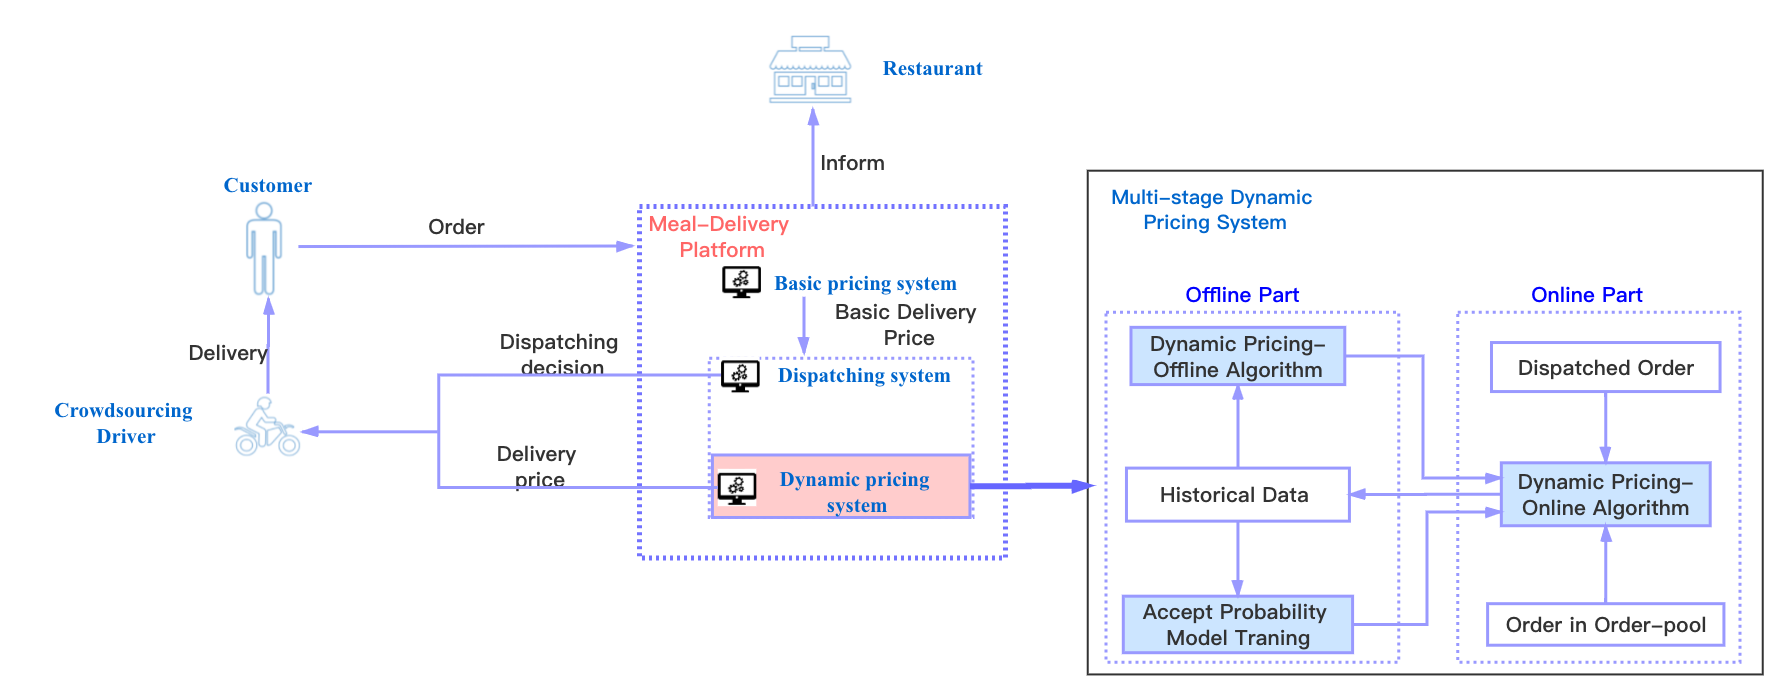
\includegraphics[width=\columnwidth]{teaser.png}
  \caption{The Framework of multi-stage Dynamic Pricing}
  \label{fig:teaser}
\end{teaserfigure}

%%
%% This command processes the author and affiliation and title
%% information and builds the first part of the formatted document.
\maketitle

\section{Introduction}
 The restaurant meal-delivery is going through the explosive growth as this service becomes more and more fashionable. Take Meituan Dianping, the most popular Chinese meal-delivery platform, as an example, around 30 million meal orders are traded everyday. The aim of the platform is to provide effective and efficient service at lower delivery cost. 
 
In reality, proper delivery pricing strategy is vital for multiple stakeholders: the customers, the crowdsourcing drivers, the restaurants, and the meal-delivery platform. As shown in Figure \ref{fig:profit}, higher delivery price means descent income for the drivers, more orders delivered, higher quality of user experience and less food wasting for the restaurants. Therefore, how to price the delivery service is proposed in order to balance the profits of all the stakeholders. 

%It is worth mentioning that, for convenience "accept probability" means both the probability of a order being accepted in the dispatching stage and the probability of a order undertook in the order-pool stage.
A typical process in the meal-delivery problem is depicted in Figure \ref{fig:flowchart}. After a customer orders the meal through Meituan APP, the meal-delivery platform starts to work. Firstly, the basic pricing system would determine a basic delivery price for the order based on the property of the order, such as the geographic locations of the restaurant and the customer. Secondly, according to plentiful spatial-temporal information and the basic delivery price, the dispatching system would decide whether to dispatch the order to a driver or to put the order in the order-pool. The orders in the order-pool are presented to the surrounding drivers and they can undertake these orders on their own will. If the delivery price is not attractive enough, the order may not be accepted. In other words, it may be rejected by the designated driver or left in order-pool without anybody undertake it. Then, the order would either be re-dispatched or continue to be left in the order-pool. At last, the order would be either accepted successfully or be canceled by the system. In order to increase the chance of successful acceptation, the dynamic pricing system would adjust the delivery price once in a while(so called multi-stage dynamic pricing). 
 \begin{figure}[h]
  \centering
  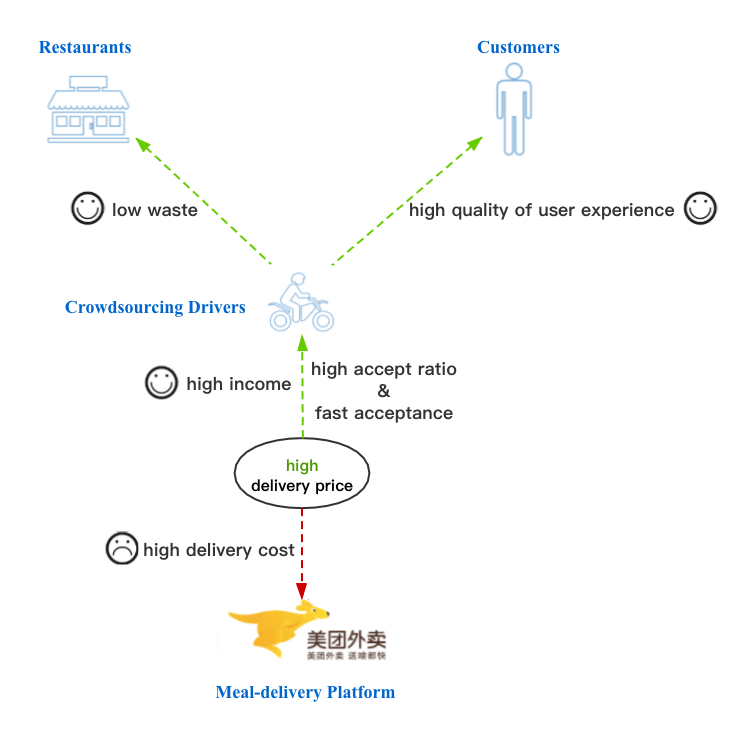
\includegraphics[width=0.3\textwidth]{profit.png}
  \caption{The impact of delivery price on each stakeholder}
  \Description{need to add description}
  \label{fig:profit}
\end{figure}
 \begin{figure}[h]
  \centering
  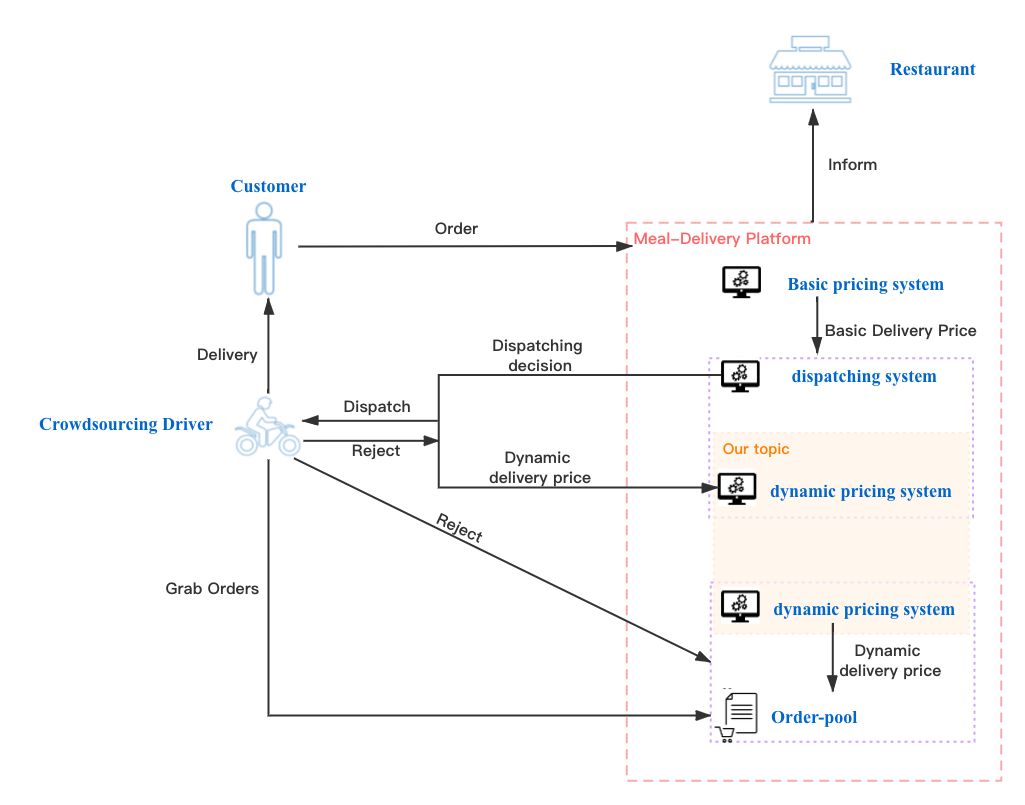
\includegraphics[width=0.4\textwidth]{flowchart.png}
  \caption{The typical process in the meal-delivery problem}
  \Description{need to add description}
  \label{fig:flowchart}
\end{figure}

 


% As we mentioned before, there are two kinds of pricing system in meal-delivery crowdsourcing. The basic pricing system make the basic delivery price only according to the property of the order itself. The dynamic pricing system involves two stages: dispatching stage and order-pool stage. Dynamic pricing in the dispatching stage makes price adjustment according to the dispatching decision. Specifically, the information of the matched driver is given, such as the geographical location of the driver, the delivery already accepted by the driver, the traveling speed and so on. Dynamic pricing in the order-pool stage would makes price adjustment of the delivery if it is pushed into the order-pool according to the context information such as the number of available drivers and their historical behavior.
%There are some researches on pricing in traditional crowdsourcing\cite{singer2013pricing,singla2013truthful}, in which the drivers are enough so that all the orders could be completed. Recently, spatial crowdsourcing platform is emerging, such as Uber and DiDi, where the driver only take one order at once. The unified market in traditional crowdsourcing tends to fragment into multiple local markets in spatial crowdsourcing. As a result of the spatiotemporal distributions of workers and orders, each local market often varies in supply and demand, posing a need for dynamic pricing for each local market. In other words, dynamic pricing for spatial crowdsourcing provides a unified price for each local market. However, it is unreasonable to make a unified delivery price for all the orders in a local market for meal-delivery problem. In meal-delivery, a driver can take multiple orders simultaneously. The accept probability is influenced by a lot of factors, such as the geographical location of the dispatched driver(dispatching stage)/surrounding drivers(order-pool stage), the accepted orders of the driver(s) and the new order. Therefore, it is necessary to make dynamic pricing for each order.
 
In this paper, we deal with the multi-stage dynamic pricing problem(MSDP, for short) for the meal-delivery platform. In reality, an estimated arrival time(ETA) is posed on each order and is linked to the driver's salary. Therefore, as time goes by, the timeout rate of an order increases such that the possibility it being accepted decreases. Therefore, before the order being accepted, the pricing decision is supposed to be changed multiple times as time flows, i.e., multi-stage pricing. Let $N$ be the order set placed during the week/month. The order not being accepted in former pricing stage would be transited to the next pricing stage. The orders could be pricing $|T|$ times at most before being accepted by the drivers. As orders continue to be accepted, the order set continue to be decreased. As shown in Figure \ref{fig:orders}, the size of the circle represents the size of the remained order set. $N_{t_0}$ means the order set transited to pricing stage $t_0$. Normally, the time interval between two pricing stages is a constant range from 1 to 10 minutes.
\begin{figure}[h]
  \centering
  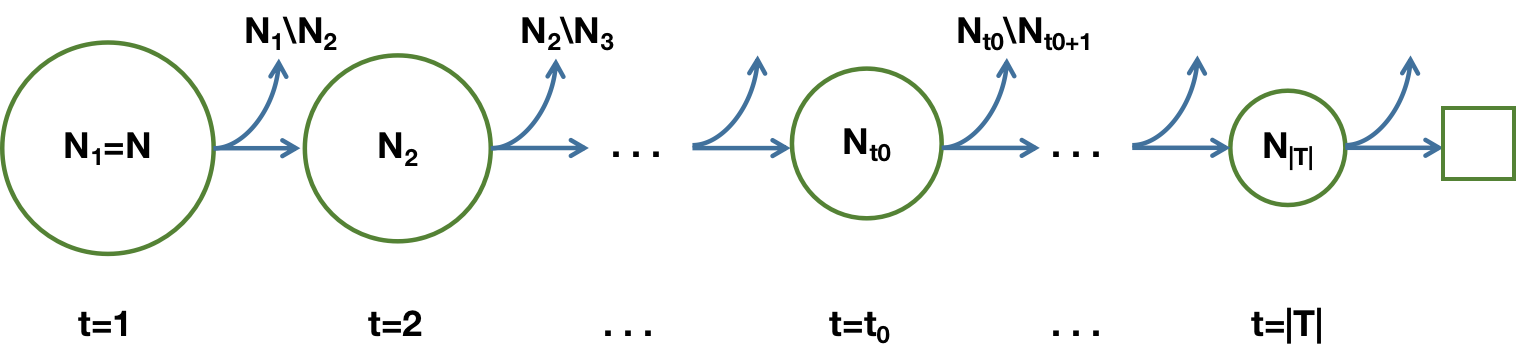
\includegraphics[width=0.5\textwidth]{orders.png}
  \caption{The transition of the orders}
  \Description{need to add description}
  \label{fig:orders}
\end{figure}
To the best of our knowledge, we deal with the MSDP for meal-delivery platform for the first time that is not trivial due to the following three challenges.
\begin{itemize}
\item The problem involves multiple stages and multiple stakeholders, how to formulate the MSDP to balance the interest of the multiple stakeholders is very fundamental.
\item We introduce a semi-black-box model to forecast the relationship between the accept probability of an order and the delivery price. However, it induces the mathematical formulation non-linear and non-convex so that the formulation is intractable.
\item There are two challenges to make delivery price decision by solving the model in real-time: 1. we need to make the pricing decision in real time whereas the total delivery cost should be controlled within limited weekly/monthly budget; 2. the delivery price decision of an order needs to be performed in few milliseconds.
\end{itemize}
%In summary, we focus on dynamic pricing of the meal-delivery crowdsourcing in this paper. We aim to optimize the delivery price by maximizing the total accept probabilities of all the orders. The delivery price of each order is supposed to be limited within an upper and lower bound. To this end, in the beginning, two machine learning models are used to predict the accept probability distribution of each order in dispatching stage and order-pool stage respectively. We would not discuss the machine learning models in detail but provide the experimental result comparisons in the later section. After the accept probability distributions are given, we can formulate the dynamic pricing problem as a non-convex programming model. In general, a non-convex model is intractable, so that we need to simplify it into a tractable one. Through analysis on the historical data, we discover that it is possible to approximate the model to a convex programming model. It is computationally expensive to solve the model online exactly. Therefore, we originally propose an offline-online method to solve the mathematical model.
The contribution of this work is summarized as follows:
\begin{itemize}
\item We formally propose a framework of MSDP for mean-delivery platform. We formulate the MSDP as a non-convex optimization problem based on a semi-black-box forecasting model which reflects the relationship between the accept probability of an order and the delivery price.
\item To make the real-time pricing decision for each order, we propose an offline-online algorithm. Firstly, in offline part, We calculate the empirical Lagrangian Multiplier for each pricing stage based on the historical data set. Secondly, the results attained in offline part are used to calculate a proper delivery price for each order in online part. This algorithm helps to make quick decision in real time. Both offline experiments and online A/B tests verify the effectiveness of the algorithm.
\item As for the offline part, we propose a dynamic programming algorithm. With this algorithm, we solve a non-convex optimization for each single pricing stage repeatedly. Refer to \cite{zhao2019unified}, we reformulate the single-stage pricing problem into a convex optimization.
\item Our framework of multi-stage dynamic pricing problem is easy to implement and is applied to Meituan meal-delivery platform successfully. Through Online A/B tests, the number of canceled orders is reduced by more than 30\%.
\end{itemize}
The remainder of this paper is organized as follows: Section \ref{sec:Literature} presents a brief review of the existing work related to our proposed problem. In Section \ref{sec:desc}, we firstly describe our problem and present a formal mathematical formulation. Section \ref{sec:alg} introduces an offline-online algorithm to solve the model based on Dynamic Programming and Lagrangian Dual Theory. In Section \ref{sec:exp}, we report on the computational results. At last, we conclude the paper in Section \ref{sec:conc}.

\section{Literature Review}\label{sec:Literature}
\subsection{Dynamic Pricing for Delivery Problem or Ride-hailing Problem}
Some researches have been done about the dynamic pricing for attended home delivery \cite{klein2018model,koch2020route,yang2016choice} in which they using time slot pricing to influence customers' bookings dynamically based on approximate dynamic programming. Reference \cite{yang2016choice} propose approximating the opportunity cost by calculating the insertion cost of a incoming request based on the insertion heuristic algorithm. Klein et al.\cite{klein2018model} improve the method of Yang et al. by considering expected future demand, making the delivery cost approximation more accurate and linking the most current information about already accepted customers. Koch et al. \cite{koch2020route} combine and extend the methods in previous paper by considering limited fleet size, more flexible customer choice and dynamic vehicle routing with time windows. The approximate dynamic programming method would suffer from curse of dimensionality, which could not satisfy the strict computational time requirements. Some other papers deal with the dynamic pricing of the same-day delivery problem. Ulmer \cite{ulmer2020dynamic} establishes a markov decision process model for dynamic routing and pricing of same-day delivery and presents anticipatory pricing and routing policy method to solve it. Based on the work of Ulmer \cite{ulmer2020dynamic}, Prokhorchuk et al. \cite{prokhorchuk2019stochastic} consider stochastic travel time to make the model more applicable. 
\subsection{Dynamic Pricing for Ride-hailing Problem}
There are some literature involved in dynamic pricing for ride-hailing platforms. For dynamic pricing for ride-hailing platforms, the main aim is to maximize the total revenue of the platform considering the imbalance between the demand(number of the passengers) and the supply(the number online drivers). Some ride-hailing platforms uses the dynamic pricing strategy called surge/prime pricing, in which the base fare is multiplied by a multiplier that is greater than one when the demand is very high relative to supply\cite{hall2015effects}. Castillo et al.\cite{castillo2017surge} proposed a steady-state model for dynamic pricing in ride-hailing, and validates that dynamic pricing is particularly important for ride-hailing due to the so-called wild goose chase phenomenon. Zha et al.\cite{zha2018geometric} built a spatial pricing model based on a discrete-time geometric matching framework where a customer is matched to her closest available vehicle within a certain radius. They presented spatial pricing assuming a revenue-maximizing platform and considering both the short- and long-run labor supply. Tong et al. \cite{tong2018dynamic} proposed the Global Dynamic Pricing (GDP) in spatial crowdsourcing in a ride-hailing platform context. It aims to deal with dynamic pricing in multiple local markets with  unknown demand, limited supply and dependent supply. However, we discovered two differences of pricing between ride-hailing and meal delivery problem. On one hand, dynamic pricing for ride-hailing determines the price presented to passengers temporally and spatially, but for meal delivery, we make delivery price presented to drivers case by case based on the features of the orders and matched(or available) drivers. On the other hand, the aim of dynamic pricing for ride-hailing is maximize the revenue of the platform, but for meal delivery, we maximize the total accept probability of all the orders within the limited budget.

\subsection{Real-time Bidding for advertisement display}
There is another topic related to dynamic pricing for meal-delivery problem which is called real-time bidding(RTB) for advertisement display. RTB determine the bidding price for the advertisers to win on a display ad impression in real time. The aim of RTB is to maximize the KPIs (such as click-through rate, click-conversion rate (CTR/CVR) and so on) within limited budget. Perlich et al. \cite{perlich2012bid}first proposed a linear bidding function based on impression evaluation, which has been widely used in real-word applications. Later on, Zhang et al. \cite{zhang2014optimal} derive the non-linear relationship between the impression level evaluation and the optimal bid. Lee et al. \cite{lee2013real} formulate the real-time bidding as an online linear programming which optimize the performance metrics while satisfying the so called smooth delivery constraint. The smooth delivery constraint is used to have sustainable influence on the ads and avoid pushing large amount of ads in peak-hour which maybe degrade the performance. Cai et al. \cite{cai2017real} formulate the bid decision process as a reinforcement learning problem and solve the problem by dynamic programming for small scale problem and a neural network is used to generalize the solution to the large scale problem. Wang et al. \cite{wang2017ladder} optimize the real-time bidding without limited budget using deep reinforcement learning, specifically DQN. They only make the decision for one single advertiser at once and its competitors as part of the environment. Jin et al. \cite{jin2018real} propose a multi-agent reinforcement learning framework which treat all the advertisers equally. The differences between real-time bidding and dynamic pricing for meal-delivery problem focus on two points. Firstly, the meal-delivery platform does not have competitors when they present the delivery price to the riders which the advertiser have in real-time bidding problem. Secondly, the objective of dynamic pricing for meal-delivery problem is to maximize the accept probability which is positively related to the delivery price. In contrast, the objective of real-time bidding problem is to maximize the CTR/CVR which scarcely has direct connection with the bidding price.

\section{Problem Description and Mathematical Formulation}\label{sec:desc}

\subsection{Accept Probability Model Forecasting}\label{sec:pro-model}
 As we mentioned before, the aim of MSDP is to maximize the number of accepted orders. In order to formulate this, our objective function is to maximize the expected value of the number of accepted orders based on the accept probability of the orders. With multiple pricing stages, if an order is not accepted in a former pricing stage, it would be transited to the next pricing stage. The transition process of an order is illustrated in Figure \ref{fig:ordertran}. Each node presents a pricing stage. Let $p_1$ be the accept probability in the first pricing stage. Correspondingly, $1-p_1$ is the probability transited to the second pricing stage. Consequently, the accept probability after pricing stage $|T|$ is $\prod_{t_0=1}^{|T|-1}(1-p_{t_0})p_{|T|}$. Otherwise, the order would be canceled with the probability of $\prod_{t_0=1}^{|T|}(1-p_{t_0})$. In total, the probability of an order being accepted is expressed in following:
\begin{equation}
    p=\sum_{t=1}^{|T|}\prod_{t_0=1}^{t-1}(1-p_{t_0})p_{|T|}
\end{equation}
%Here, we also define $b$ as average budget per order(average budget for short) which is used in Section \ref{sec:alg} 
\begin{figure}[h]
  \centering
  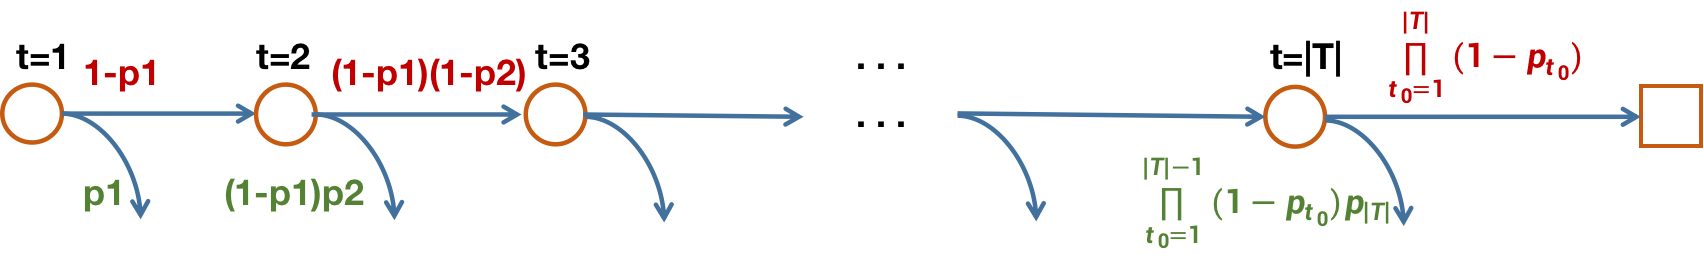
\includegraphics[width=0.5\textwidth]{transit.png}
  \caption{The transition process of an order}
  \Description{need to add description}
  \label{fig:ordertran}
\end{figure}
In order to make optimal delivery pricing decision for each order, we need to forecast the relationship between accept probability and delivery price. Although black-box forecasting method, such as neural networks, have been widely used in many applications, there are still gaps between the black-box model and pricing decision making. Instead, in this paper, we use a semi-black-box forecasting method. We assume that the accept probability model conforms to the following logistic function:
\begin{align}
    \label{eq1.4} & p_{i,t}(c)=\frac{1}{1+e^{\alpha_{i,t} c+\beta_{i,t}}}
\end{align}
Meanwhile, $\alpha_{i,t}$ and $\beta_{i,t}$ are the parameters trained by the machine learning, such as neural networks. Note that $\alpha_{i,t}$ should be less than 0 in order to ensure the function monotonically increasing. The accept probability model of the orders is illustrated in Figure \ref{fig:two orders}. As we can see, the accept probabilities of the two orders might be different largely even though their delivery prices are the same. The accept probability of order A (over 95\%) is much higher than that of order B(about 45\%) when the dynamic price adjustment is 0. Therefore, the motivation is to increase the total accept probability by moving 2 units of the delivery price from order A to order B.

\begin{figure}[h]
  \centering
  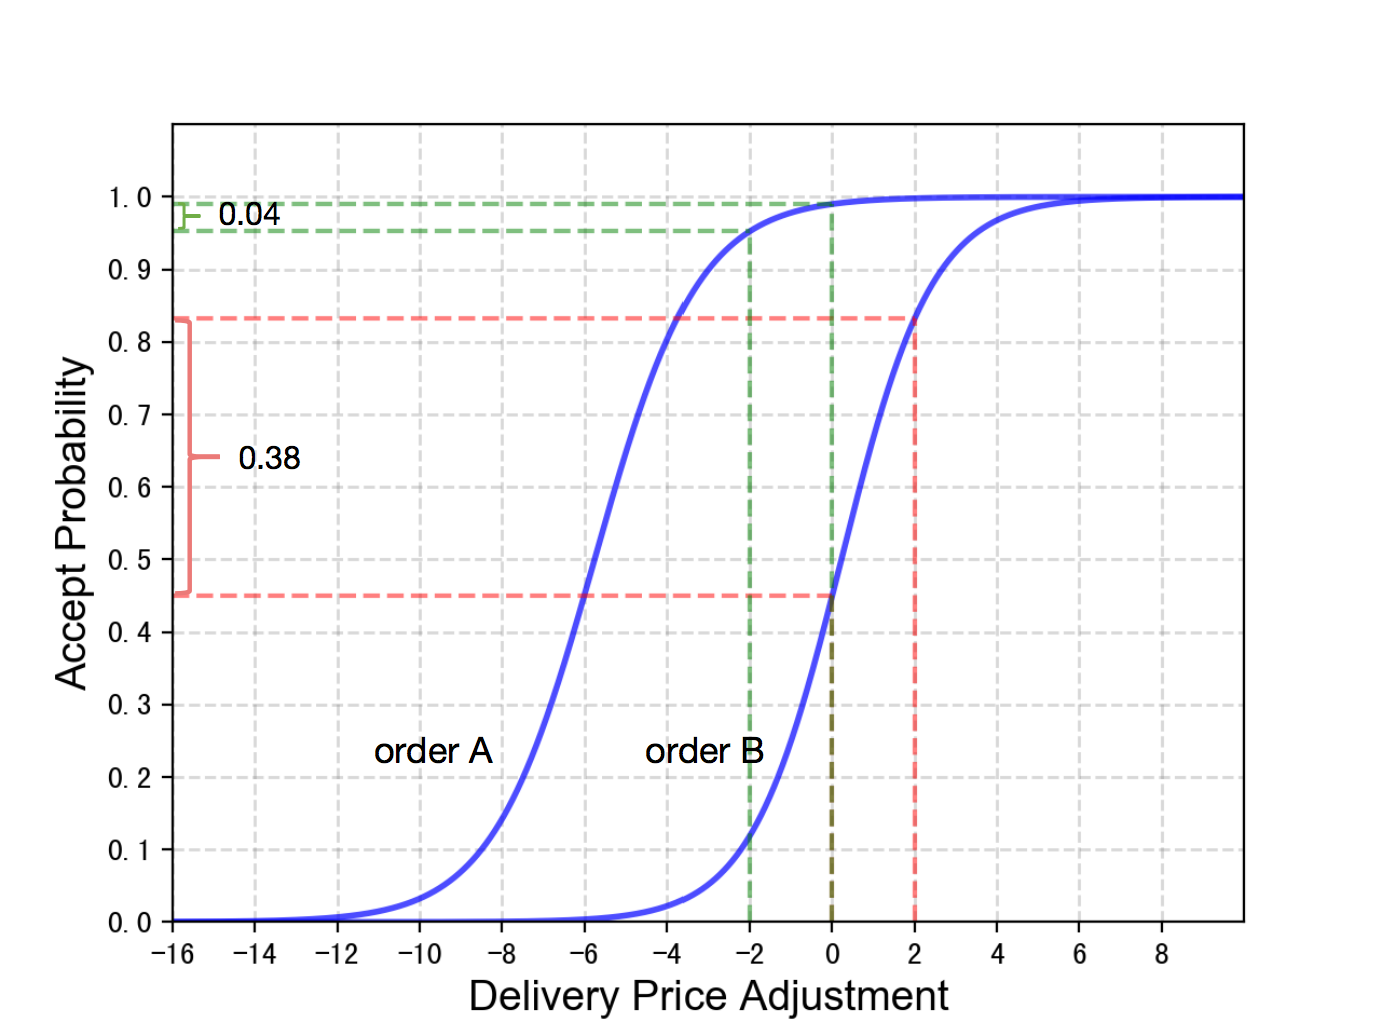
\includegraphics[width=0.49\textwidth]{two orders.png}
  \caption{The relationship between the delivery price and accept probability}\label{fig:two orders}
  \Description{need to add description}
\end{figure}

\subsection{Definition and Mathematical Model}
The set $N$ consists of the order placed within a week/month. The set $T$ means the pricing stage set, i.e., an order could be priced at most $|T|$ times. The decision variable $c_{i,t}$ means the delivery price adjustment of the order $i\in N$ at stage $t\in T$. $c_{i,t}$ can be negative or positive, in which negative means a delivery price discount and positive means an increase in delivery price. The function $p_{i,t}(c_{i,t})$ denote the accept probability model of the order $i\in N$ if it is transited to pricing stage $t\in T$. The price adjustment should be between the upper bound $C_i^u$ and lower bound $C_i^l$ with $C_i^l\le0$ in general. The expected value of the total delivery cost should be within the given budget $B$.

The MSDP can be modeled as follows:
\begin{align}
    \label{eq1.1}\max~& \sum_{i\in N}\sum_{t\in T}(\prod_{t_0=1}^{t-1} (1-p_{i,t_0}(c_{i,t_0})))p_{i,t}(c_{i,t}) \\
    \label{eq1.2}\mbox{s.t. }& \sum_{i\in N}\sum_{t\in T}(\prod_{t_0=1}^{t-1} (1-p_{i,t_0}(c_{i,t_0})))p_{i,t}(c_{i,t})c_{i,t}\le B\\
    \label{eq1.3}& C_i^l\le c_{i,t}\le C_i^u & \forall i \in N, t \in T
\end{align}
The objective function \eqref{eq1.1} maximizes total accept probability, i.e., the excepted value of the accepted order quantity. Constraints \eqref{eq1.2} represents that the total expected value of the total delivery cost should be within the given budget B. Constraints \eqref{eq1.3} restrain the delivery price $c_{i,t}$ within the given upper and lower bound.

\section{Algorithm}\label{sec:alg}
In reality, we need to make a pricing decision in real time and control the delivery cost within a weekly/monthly budget. However, we are not able to attain all the information of the order placed during the week/month. Therefore, how to control the total cost within the limited budget and make full use of the budget is the key to solving the problem. In this paper, we introduce an offline-online algorithm to solve it. At first, we come up with a dynamic programming algorithm to solve the model presented in Section \ref{sec:desc} offline based on the historical data set. The offline algorithm helps to calculate the empirical Lagrangian Multiplier $\lambda^*_t$ for the pricing stage $t$. Then, $\lambda^*_t$ would be used to make real-time pricing decision online.
\subsection{Dynamic Programming Formulation}
Let $N_{\tilde{t}}$ be the remained order set transited to pricing stage $\tilde{t}$ if there is no budget posed on stage 1 to $\tilde{t}-1$. Thinking of the right-hand side of the constraint \eqref{eq1.2} $\tilde{B}$ taking value 0, 1, 2,...,B as "state", and the pricing stage subset $\{\tilde{t},\tilde{t}+1,...,|T|\}$ represented by $\tilde{t}$ as the "stage"(Note that this "stage" is used to define a sub-problem of dynamic programming which is different from pricing stage we mentioned before), leads us to define the sub-problem $P_{\tilde{t}}(\tilde{B})$ and the optimal value function $G_{\tilde{t}}(\tilde{B})$ as follows:
\begin{align}
    \label{eq2.1}G_{\tilde{t}}(\tilde{B})= \max~& \sum_{i\in N_{\tilde{t}}}\sum_{t=\tilde{t}}^{|T|}(\prod_{t_0=\tilde{t}}^{t-1} (1-p_{i,t_0}(c_{i,t_0})))p_{i,t}(c_{i,t}) \\
    \label{eq2.2}\mbox{s.t. }& \sum_{i\in N_{\tilde{t}}}\sum_{t=\tilde{t}}^{|T|}(\prod_{t_0=\tilde{t}}^{t-1} (1-p_{i,t_0}(c_{i,t_0})))p_{i,t}(c_{i,t})c_{i,t}\le \tilde{B}\\
    \label{eq2.3}& C_i^l\le c_{i,t}\le C_i^u  ,\forall i \in N_{\tilde{t}}, t=\tilde{t},\tilde{t}+1,...,|T|
\end{align}
  Then, $z=G_{1}(B)$ gives us the optimal value of the MSDP\cite{wolsey1998integer}. 
  
  In order to define a recursion that allows us calculate $G_{\tilde{t}}(\tilde{B})$ in terms of $G_{s}(\tilde{B_0})$ for $s>\tilde{t}$ and $\tilde{B_0} \le \tilde{B}$, We need to define a single-stage pricing problem with the objective value function $g_{\tilde{t}}(\tilde{B})$ where the budget $\tilde{B}$ is only spent on a single stage $\tilde{t}$. It indicates the optimal expected value of accepted order quantity if the budget $\tilde{B}$ is spent on a single stage $\tilde{t}$. Function $g_{\tilde{t}}(\tilde{B})$ is expressed in following:
\begin{align}
    \label{eq3.1}g_{\tilde{t}}(\tilde{B})= \max~& \sum_{i\in N_{\tilde{t}}}p_{i,\tilde{t}}(c_{i,\tilde{t}}) \\
    \label{eq3.2}\mbox{s.t. }& \sum_{i\in N_{\tilde{t}}}p_{i,\tilde{t}}(c_{i,\tilde{t}})c_{i,\tilde{t}}\le \tilde{B}\\
    \label{eq3.3}& C_i^l\le c_{i,\tilde{t}}\le C_i^u & \forall i \in N_{\tilde{t}}
\end{align}


Let $\Delta_{\tilde{t}}(\tilde{B})$ denotes the accepted orders increment at stage $\tilde{t}$ brought by budget $\tilde{B}$, then
\begin{equation}
    \Delta_{\tilde{t}}(\tilde{B})=g_{\tilde{t}}(\tilde{B})-g_{\tilde{t}}(0)
\end{equation}
In other words, there are about $\Delta_{\tilde{t}}(\tilde{B})$ orders not being transited to stage $\tilde{t}+1$. Then the remained order quantity of $\tilde{t}+1$ would be reduced to
 $|N'_{\tilde{t}+1}|=|N_{\tilde{t}+1}|- \Delta_{\tilde{t}}(\tilde{B})$. 
What can we say about optimal solution for problem $P_{\tilde{t}}(\tilde{B})$ with value $G_{\tilde{t}}(\tilde{B})$? Clearly, we can get it by an optimal budget combination on a single pricing stage $\tilde{t}$ and the pricing stage set $\{\tilde{t}+1,...,|T|\}$. 

 In order to simplify the solution process, we make the following assumption:
 %The optimal average accept probability for $N_{\tilde{t}}$ is $\frac{G_{\tilde{t}}(\tilde{B})}{N_{\tilde{t}}}$ if the average budget is $\frac{\tilde{B}}{N_{\tilde{t}}}$. 
 \newtheorem{assumption}{Assumption}
\begin{assumption}
The average optimal value is independent to the order set $N_{\tilde{t}}$ and is only related to the dynamic pricing stage set $\{\tilde{t},\tilde{t}+1,...,|T|\}$ and the average budget $\tilde{b}$. 
\end{assumption}
Then, we introduce $\bar G_{\tilde{t}}(\tilde{b})$ as average optimal value which can be calculated with following :
\begin{equation}
    \bar G_{\tilde{t}}(\tilde{b})=\frac{G_{\tilde{t}}(\tilde{b}*|N_{\tilde{t}}|)}{|N_{\tilde{t}}|}
\end{equation}
Meanwhile, $\tilde{b}$ is the average budget of each order.

Therefore, the recursion can be represented as follows:
\begin{equation}\label{eqr1.1}
\begin{aligned}
    G_{\tilde{t}}(\tilde{B})&=\max_{k=0,1,...,\tilde{B}}\{g_{\tilde{t}}(k)+|N'_{\tilde{t}+1}|*\bar G_{\tilde{t}+1}(\frac{\tilde{B}-k}{|N'_{\tilde{t}+1}|})\}\\
    &=\max_{k=0,1,...,\tilde{B}}\{g_{\tilde{t}}(k)+\frac{|N'_{\tilde{t}+1}|}{|N_{\tilde{t}+1}|}* G_{\tilde{t}+1}[(\tilde{B}-k)\frac{|N_{\tilde{t}+1}|}{|N'_{\tilde{t}+1}|}]\}
\end{aligned}
\end{equation}
Now starting the recursion with $G_{|T|}(\tilde{B})=g_{|T|}(\tilde{B})$ for $\tilde{B} \ge 0$, we then use the recursion \eqref{eqr1.1} to successively calculate $G_{|T|-1},G_{|T|-2},...,G_1$ for all integral values of $\tilde{B}$ from 0 to B. An overview of the dynamic programming algorithm is depicted in Algorithm \ref{alg:DP}. In this process, we need to solve a single-stage pricing problem with objective value of $g_{\tilde{t}}(\tilde{B})$ for all $\tilde{t}\in T$ and $\tilde{B}\in \{0,1,2,...,B\}$. 

\begin{algorithm}[t]
\DontPrintSemicolon
 \SetKwComment{Comment}{$\triangleright$\ }{}
 \SetKw{KwBy}{by}
   \SetNoFillComment
    \caption{Dynamic Programming}\label{alg:DP}
        \KwIn{Pricing stage set $T$, order set $N_{\tilde{t}}, \forall t\in T$, total budget B} 
        \KwOut{empirical Lagrangian Multipliers $\lambda^*[|T|]$} 
        \BlankLine
        \BlankLine
        \Comment*[l]{Solve the single-stage pricing problems repeatedly and record the solutions in arrays $g[|T|][B]$ and $\lambda[|T|][B]$}
        \ForAll{$\tilde{t}\in T$}{
        \While{$\tilde{B}$<=B}{
        $g[\tilde{t}][\tilde{B}],\lambda[\tilde{t}][\tilde{B}]\gets BA(N_{\tilde{t}},\tilde{B})$\;
        $\tilde{B}\gets \tilde{B}+1$\;
        }
        }
        \BlankLine
        \BlankLine
        \Comment*[l]{Solve the sub-problem $P_{\tilde{t}}(\tilde{B})$ recursively and record the optimal solution in the array G[|T|][B]}
        $G[|T|] \gets g[|T|]$\;
        $\tilde{t}\gets |T|-1$\;
        $\tilde{B}\gets 0$\;
        \While{$\tilde{t}\ge 1$}{
        \While{$\tilde{B}$<=B}{
        $G[\tilde{t}][\tilde{B}]\gets G[\tilde{t}+1][\tilde{B}]$\;
        $k^*\gets 0$\;
        \For{$k\gets0$ \KwTo $\tilde{B}$ \KwBy $1$}{
        $\Delta \gets g[\tilde{t}][k]-g[\tilde{t}][0]$\;
        $N'\gets N_{\tilde{t+1}}-\Delta$\;
        $temp\gets g[\tilde{t}][k]+\frac{N'}{N}G[\tilde{t}+1][\lfloor{\frac{N}{N'}(\tilde{B}-k)}\rfloor]$\;
        \If{$G[\tilde{t}][\tilde{B}]< temp$}{$G[\tilde{t}][\tilde{B}]\gets temp$\;
        $k^*\gets k$\;
        }
        }
        $a[\tilde{t}][\tilde{B}]\gets k^*$\Comment*[l]{a[][] is used to backtrack the optimal budget allocation path}
        $\tilde{B}\gets \tilde{B}+1$\;
        }
        $\tilde{t}\gets \tilde{t}-1$
        }
       \Comment*[l]{Backtrack the optimal solution and record the optimal empirical Lagrangian Multiplier for each stage into arrays $\lambda^*[|T|]$}
       $B_0 \gets B$\;
       \For{$t=1$ \KwTo $|T|$ \KwBy $1$}{
      $B^* \gets a[t][B_0]$\;
      $\lambda^*[t] \gets \lambda[t][B^*]$\; 
      $B_0 \gets B_0 -B^*$
       }
        return $\lambda^*[|T|]$
\end{algorithm}

\subsection{Solve Single-stage Pricing Problem}\label{sec:offline-single}
As defined by function \eqref{eq3.1}-\eqref{eq3.3}, both objective function and constraint function are non-convex with respect to $\boldsymbol{c}$, so that solving the problem directly is very difficult. Inspired by \cite{zhao2019unified,dong2009dynamic,li2011pricing}, we can reformulate the problem into an equivalent convex optimization problem. Because $p_{i,t}(c_{i,t})=\frac{1}{1+e^{\alpha_{i,t} c_{i,t}+\beta_{i,t}}}$, we have
\begin{equation}\label{eq4.1}
\begin{split}
     & c_{i,t}(p_{i,t})=-\frac{\beta_{i,t}}{\alpha_{i,t}}+\frac{1}{\alpha_{i,t}}(\ln(1-p_{i,t})-\ln(p_{i,t}))\\
     & p_{i,t}\in(0,1), \forall i\in N,t\in T
\end{split}
\end{equation}

Consequently, the constraint function \eqref{eq3.2} can be rewritten as the functions of $p_{i,\tilde{t}}$:
\begin{equation}
    f_{\tilde{t}}(\boldsymbol{p})=\sum_{i\in N_{\tilde{t}}}p_{i,\tilde{t}}c_{i,\tilde{t}}(p_{i,\tilde{t}})\\
\end{equation}

Refer to \cite{zhao2019unified,dong2009dynamic,li2011pricing}, $f_{\tilde{t}}(\boldsymbol{p})$ is a convex function in $\boldsymbol{p}$ for $\forall \tilde{t}\in T$. 

Therefore, the original problem \eqref{eq3.1}-\eqref{eq3.3} can be reformulated as follows:
\begin{align}
    \label{eq5.1}-g_{\tilde{t}}(\tilde{B})= \min~& -\sum_{i\in N_{\tilde{t}}}p_{i,\tilde{t}} \\
    \label{eq5.2}\mbox{s.t. }& \sum_{i\in N_{\tilde{t}}}p_{i,\tilde{t}}c_{i,\tilde{t}}(p_{i,\tilde{t}})\le \tilde{B}\\
    \label{eq5.3}& P_i^l\le p_{i,\tilde{t}}\le P_i^u & \forall i \in N_{\tilde{t}}
\end{align}
Clearly, this is a differentiable convex optimization problem with respected to $\boldsymbol{p}$ and Slater's condition holds because of $C_i^l\le 0$. Therefore, its duality gap between primal and dual objective value equals to 0\cite{boyd2004convex}.

By introducing a dual variable $\lambda$, the Lagrangian Relaxation Function of the single-stage pricing problem is represented as follows:
\begin{equation}
   \label{eqs1.1} L(\boldsymbol{p},\lambda)= ~-\sum_{i\in N_{\tilde{t}}} p_{i,\tilde{t}}+\lambda [\sum_{i\in N_{\tilde{t}}}p_{i,\tilde{t}}c_{i,\tilde{t}}(p_{i,\tilde{t}})- \tilde{B}]
\end{equation}
where $P_i^l\le p_{i,\tilde{t}}\le P_i^u $,$\forall i\in N, \lambda \in \mathbb R_+$.
Correspondingly, the Lagrangian Dual Problem can be formulated as:
\begin{equation}
    \label{eqs1.2}\max_{\lambda \in \mathbb R_+}\min_{P_i^l\le p_{i,\tilde{t}}\le P_i^u} L(\boldsymbol{p},\lambda)
\end{equation}

As we mentioned before, the primal optimal value $-g_{\tilde{t}}(\tilde{B})$ is equal to the dual optimal value due to zero duality gap. By introducing a bisection algorithm represented in Algorithm \ref{alg0}, we can get the optimal solution $\lambda_{\tilde{t}}(\tilde{B})$ and the optimal value $g_{\tilde{t}}(\tilde{B})$.


\begin{algorithm}[t]
\DontPrintSemicolon
\SetKwComment{Comment}{$\triangleright$\ }{}
 \SetKw{KwBy}{by}
   \SetNoFillComment
    \caption{Bisection Algorithm for a single stage problem(BA($N_{\tilde{t}}$,$\tilde{B}$))}\label{alg0}
        \KwIn{Order set $N_{\tilde{t}}$,  budget $\tilde{B}$} 
        \KwOut{$\lambda_t(\tilde{B})$ and $g_{\tilde{t}}(\tilde{B})$} 
        $low \gets 0$ \;
        $high \gets M$\Comment*[l]{M is a big number}
        \While{$high-low> \epsilon$}{
        $s\gets 0$\;
        $opt\gets 0$\;
        $mid \gets \frac{high+low}{2}$\;
        \ForAll{$i\in N_{\tilde{t}}$}{
        $p_{i,\tilde{t}}^* \gets \arg \min_{P_i^l\le p_{i,\tilde{t}}\le P_i^u}-p_{i,\tilde{t}}+mid*p_{i,\tilde{t}}c_{i,\tilde{t}}(p_{i,\tilde{t}})$\;
        $s\gets s+ p_{i,\tilde{t}}^*c_{i,\tilde{t}}(p_{i,\tilde{t}}^*)$\;
        $opt\gets opt- p_{i,\tilde{t}}^*$\;
        }
        \If{$s-\tilde{B}\ge 0$}{$low \gets mid $}
        \Else{$high \gets mid$}
        }
        return $\lambda_t(\tilde{B}) \gets high$, $g_{\tilde{t}}(\tilde{B})\gets -opt$
\end{algorithm}

\subsection{Online Algorithm}
Given the multiplier $\lambda^*_{\tilde{t}}$ attained by the offline algorithm for stage $\tilde{t}\in T$, the problem we need to solve online can be written as:
\begin{equation}
   \label{eqo1.1} \min_{C_i^l\le c_{i,\tilde{t}}\le C_i^u} ~\{-\sum_{i\in N_{\tilde{t}}} p_{i,\tilde{t}}(c_{i,\tilde{t}})+\lambda^*_{\tilde{t}} [\sum_{i\in N_{\tilde{t}}}p_{i,\tilde{t}}(c_{i,\tilde{t}})c_{i,\tilde{t}}]\}
\end{equation}
which is equivalent to:
\begin{equation}
   \label{eqo1.2} \min_{C_i^l\le c_{i,\tilde{t}}\le C_i^u} ~\{\sum_{i\in N_{\tilde{t}}} (\lambda^*_{\tilde{t}}p_{i,\tilde{t}}(c_{i,\tilde{t}})c_{i,\tilde{t}}-p_{i,\tilde{t}}(c_{i,\tilde{t}}))\}
\end{equation}
The above problem can be reformulated as the summation of |$N_{\tilde{t}}$| separable minimizing problems as follows:
\begin{equation}
   \label{eqo1.3} \sum_{i\in N_{\tilde{t}}} \min_{C_i^l\le c_{i,\tilde{t}}\le C_i^u}\{ (\lambda^*_{\tilde{t}}p_{i,\tilde{t}}(c_{i,\tilde{t}})c_{i,\tilde{t}}-p_{i,\tilde{t}}(c_{i,\tilde{t}}))\}
\end{equation}
Therefore, to determine the delivery price for a specific order, we only need to solve a one-dimensional problem. We can solve the optimal solution for each separated problem online easily. The optimal delivery price of a specific order $i\in N$ can be expressed as follows:
\begin{equation}
\begin{aligned}
    \label{eqo1.4}c^*_{i,\tilde{t}}&= \arg \min_{C_i^l\le c_{i,\tilde{t}}\le C_i^u} \lambda^*_{\tilde{t}}p_{i,\tilde{t}}(c_{i,\tilde{t}})c_{i,\tilde{t}}-p_{i,\tilde{t}}(c_{i,\tilde{t}})
\end{aligned}
\end{equation}
Since the number of potential delivery price is limited between $C_i^l$ and $C_i^u$, the optimization problem \eqref{eqo1.4} is easily solved by enumeration the potential delivery price. Other numerical optimization methods can be developed to solve it but we are not going to further investigate them here. Note that we can solve multiple problems in parallel here due to the primal problem can be separated into multiple independent problems.
\subsection{Computational Complexity}
In this section, we discuss the computational complexity of our offline-online algorithm. As for the offline part, we analyze the computational complexity of the bisection algorithm to solve the single-stage pricing problem and the dynamic programming algorithm to solve multi-stage pricing problem. Firstly, there are $\log_2(\frac{1}{\epsilon})$ iterations for the bisection search algorithm and the complexity of each iteration is $O(N)$. So, the complexity solving the single-stage pricing problem is $O(\log_2(\frac{1}{\epsilon})N)$. Secondly, there are three steps for the dynamic programming algorithm. At line 1-4 of Algorithm \ref{alg:DP}, we solve the single-stage pricing problem for $|T|B$ times. For each iteration, we solve a single-stage pricing problem with complexity of $O(\log_2(\frac{1}{\epsilon})N)$. So, the complexity of line 1-4 $O(\log_2(\frac{1}{\epsilon})N|T|B)$. At line 8-21, we solve the sub-problem $P_{\tilde{t}}(\tilde{B})$ recursively and the complexity is $O(|T|B^2)$. At line 23-26, the complexity of the backtracking process is $O(|T|)$. Overall, the total complexity of the offline algorithm is $O(\log_2(\frac{1}{\epsilon})N|T|B+|T|(B^2+1))$

As for the online part, the number of potential delivery price is $\frac{C^u_i-C^l_i}{\delta}$ for order $i$, where $\delta$ is the pricing interval for enumeration. Since $\frac{C^u_i-C^l_i}{\delta}$ is a constant, the complexity of making delivery price of an order online is O(1).

\section{Experiments}\label{sec:exp}

To verify the effectiveness of our method, we present results of both offline experiments and online A/B tests.

\subsection{performance of offline experiments}

In this section, we conduct several offline experiments. Our instances are based on the real-world data derived from Meituan meal-delivery platform. Without loss of generality, we choose the data sets of four cities with different typical order size over 1 week. Specifically, the data sets contain 46,978, 71,427, 120,017 and 258,612 orders, respectively. The features of the semi-black-box accept probability model include the geographical location of the driver, customer and restaurant of the order, ETA of the order, dynamic information on the supply and demand, the status of the driver (such as the plan in progress), and etc. The delivery price adjustment can be calculated between the upper and lower bound which is ruled by both business manager and the basic delivery price decided by basic pricing system. It is worth mentioning that the \textit{budget} in the figures below indicates the \textit{average budget} for each order since the latter makes the results comparable among instances with different number of orders. The typical order life cycle starts from the order placed time to order delivered time or order canceled time if no one accept it more than 50 minutes. The number of pricing stages also indicates the dynamic pricing frequency. For example, if the order life cycle is 50 minutes and the number of pricing stages is 10, then the time interval between two pricing stages is 5 minutes.

\subsubsection{performance of the single-stage pricing}

In this section, we analyze the performance of the single-stage pricing algorithm. We solve the instances aforementioned by the algorithm introduced in Section \ref{sec:offline-single}. We compare the single-stage pricing result against the unified pricing mechanism in which the same delivery price adjustment is imposed on each order. Figure \ref{fig:s-pricing} reflects the relationship between the total budget and the number of accepted order. We observe an significant increase in the quantity when the budget increases. Moreover, our single-stage pricing method brings more quantity increase than the unified pricing mechanism.

\begin{figure}[h]
  \centering
  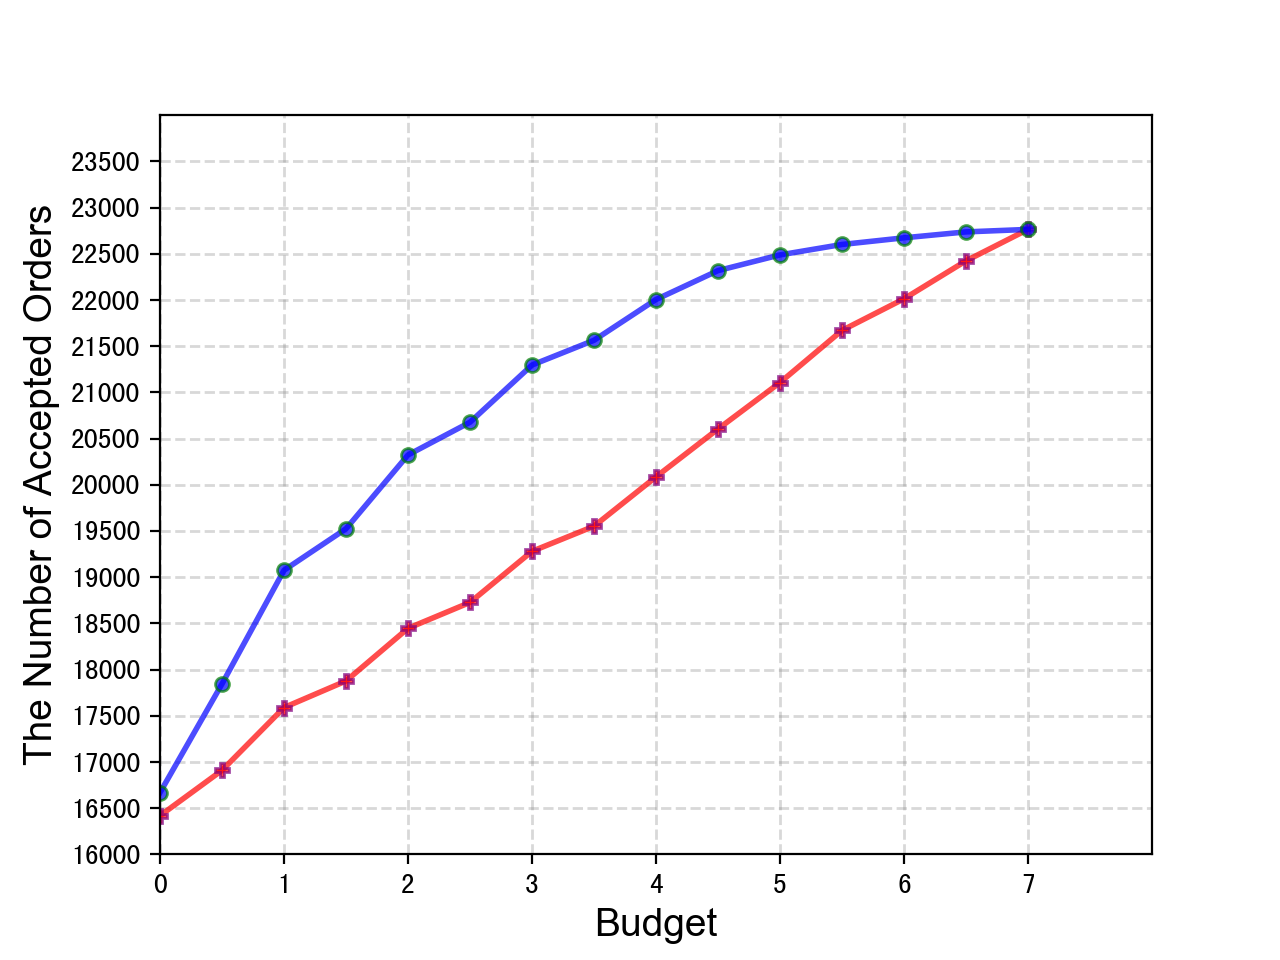
\includegraphics[width=0.49\textwidth]{s-pricing-a.png}
  \caption{Comparison between single-stage pricing and unified pricing mechanism.}\label{fig:s-pricing}
  \Description{need to add description}
\end{figure}

% \begin{figure}[tb]
%     \centering
%     \begin{subfigure}[b]{0.2\textwidth}
%     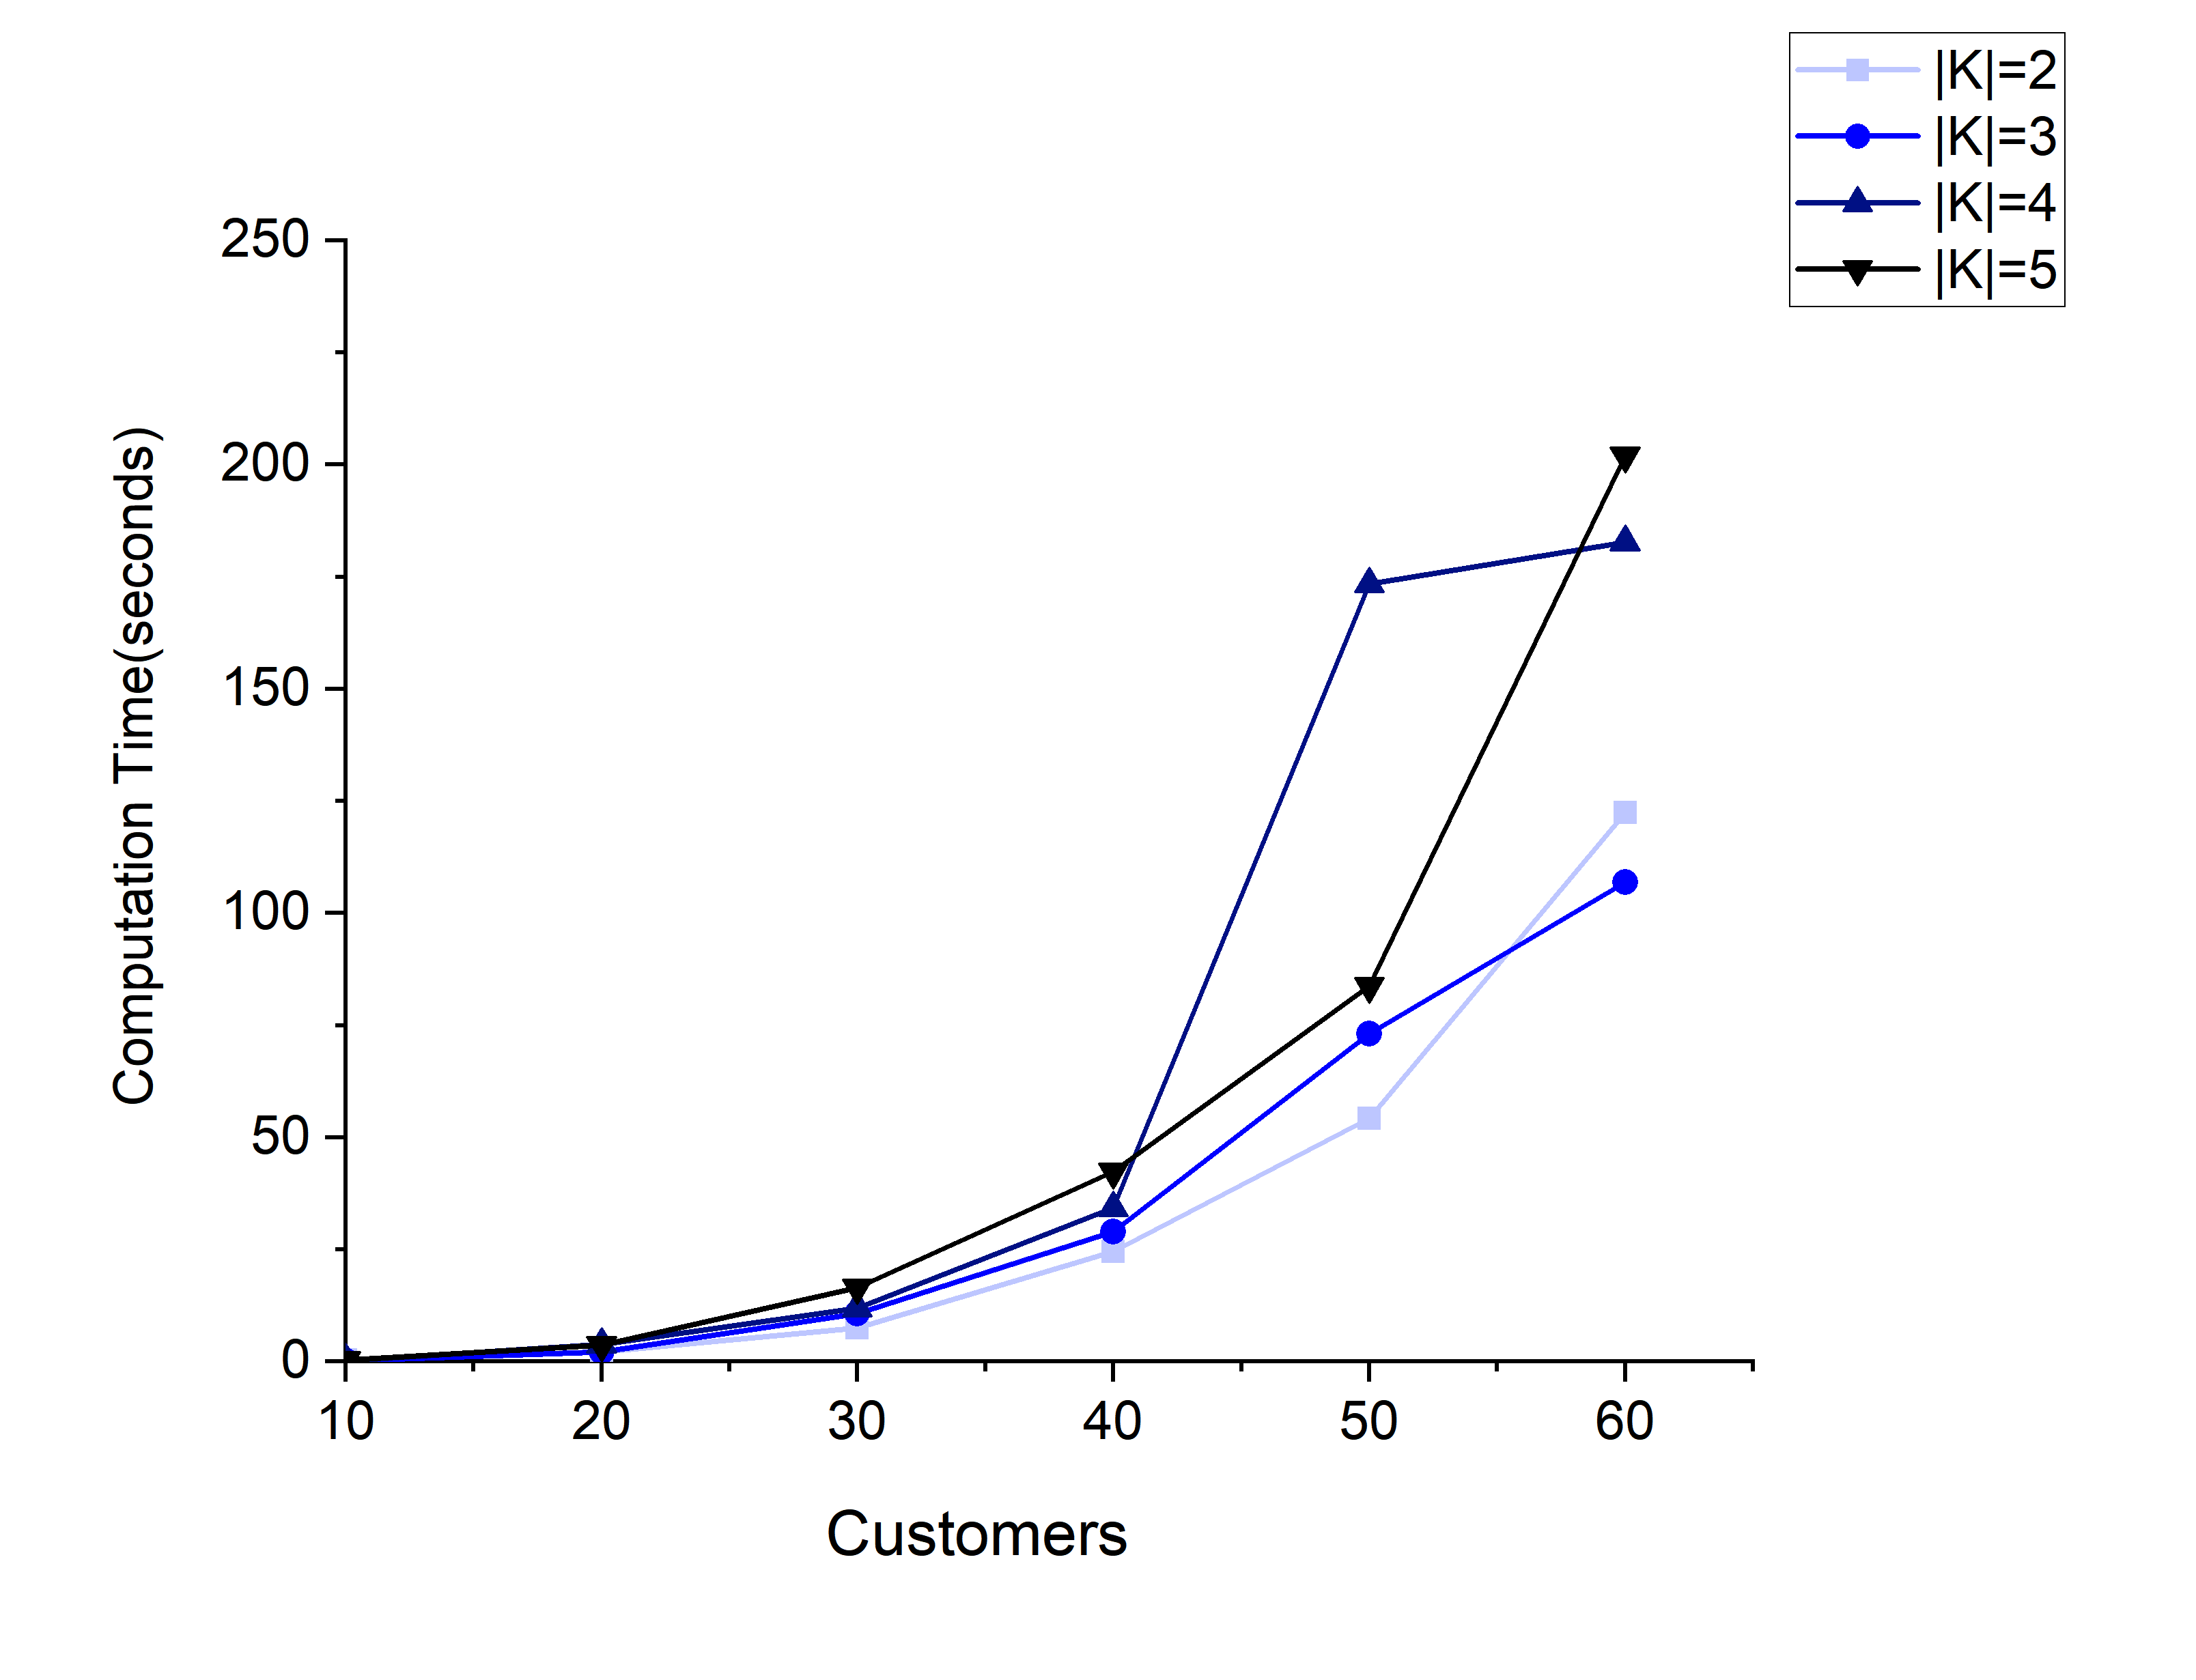
\includegraphics[width=\textwidth]{vehi_alns.png}
  
%         \caption{Number of vehicles}\label{fig:vehi_alns}
%     \end{subfigure}
%     \quad
%     \begin{subfigure}[b]{0.2\textwidth}
%     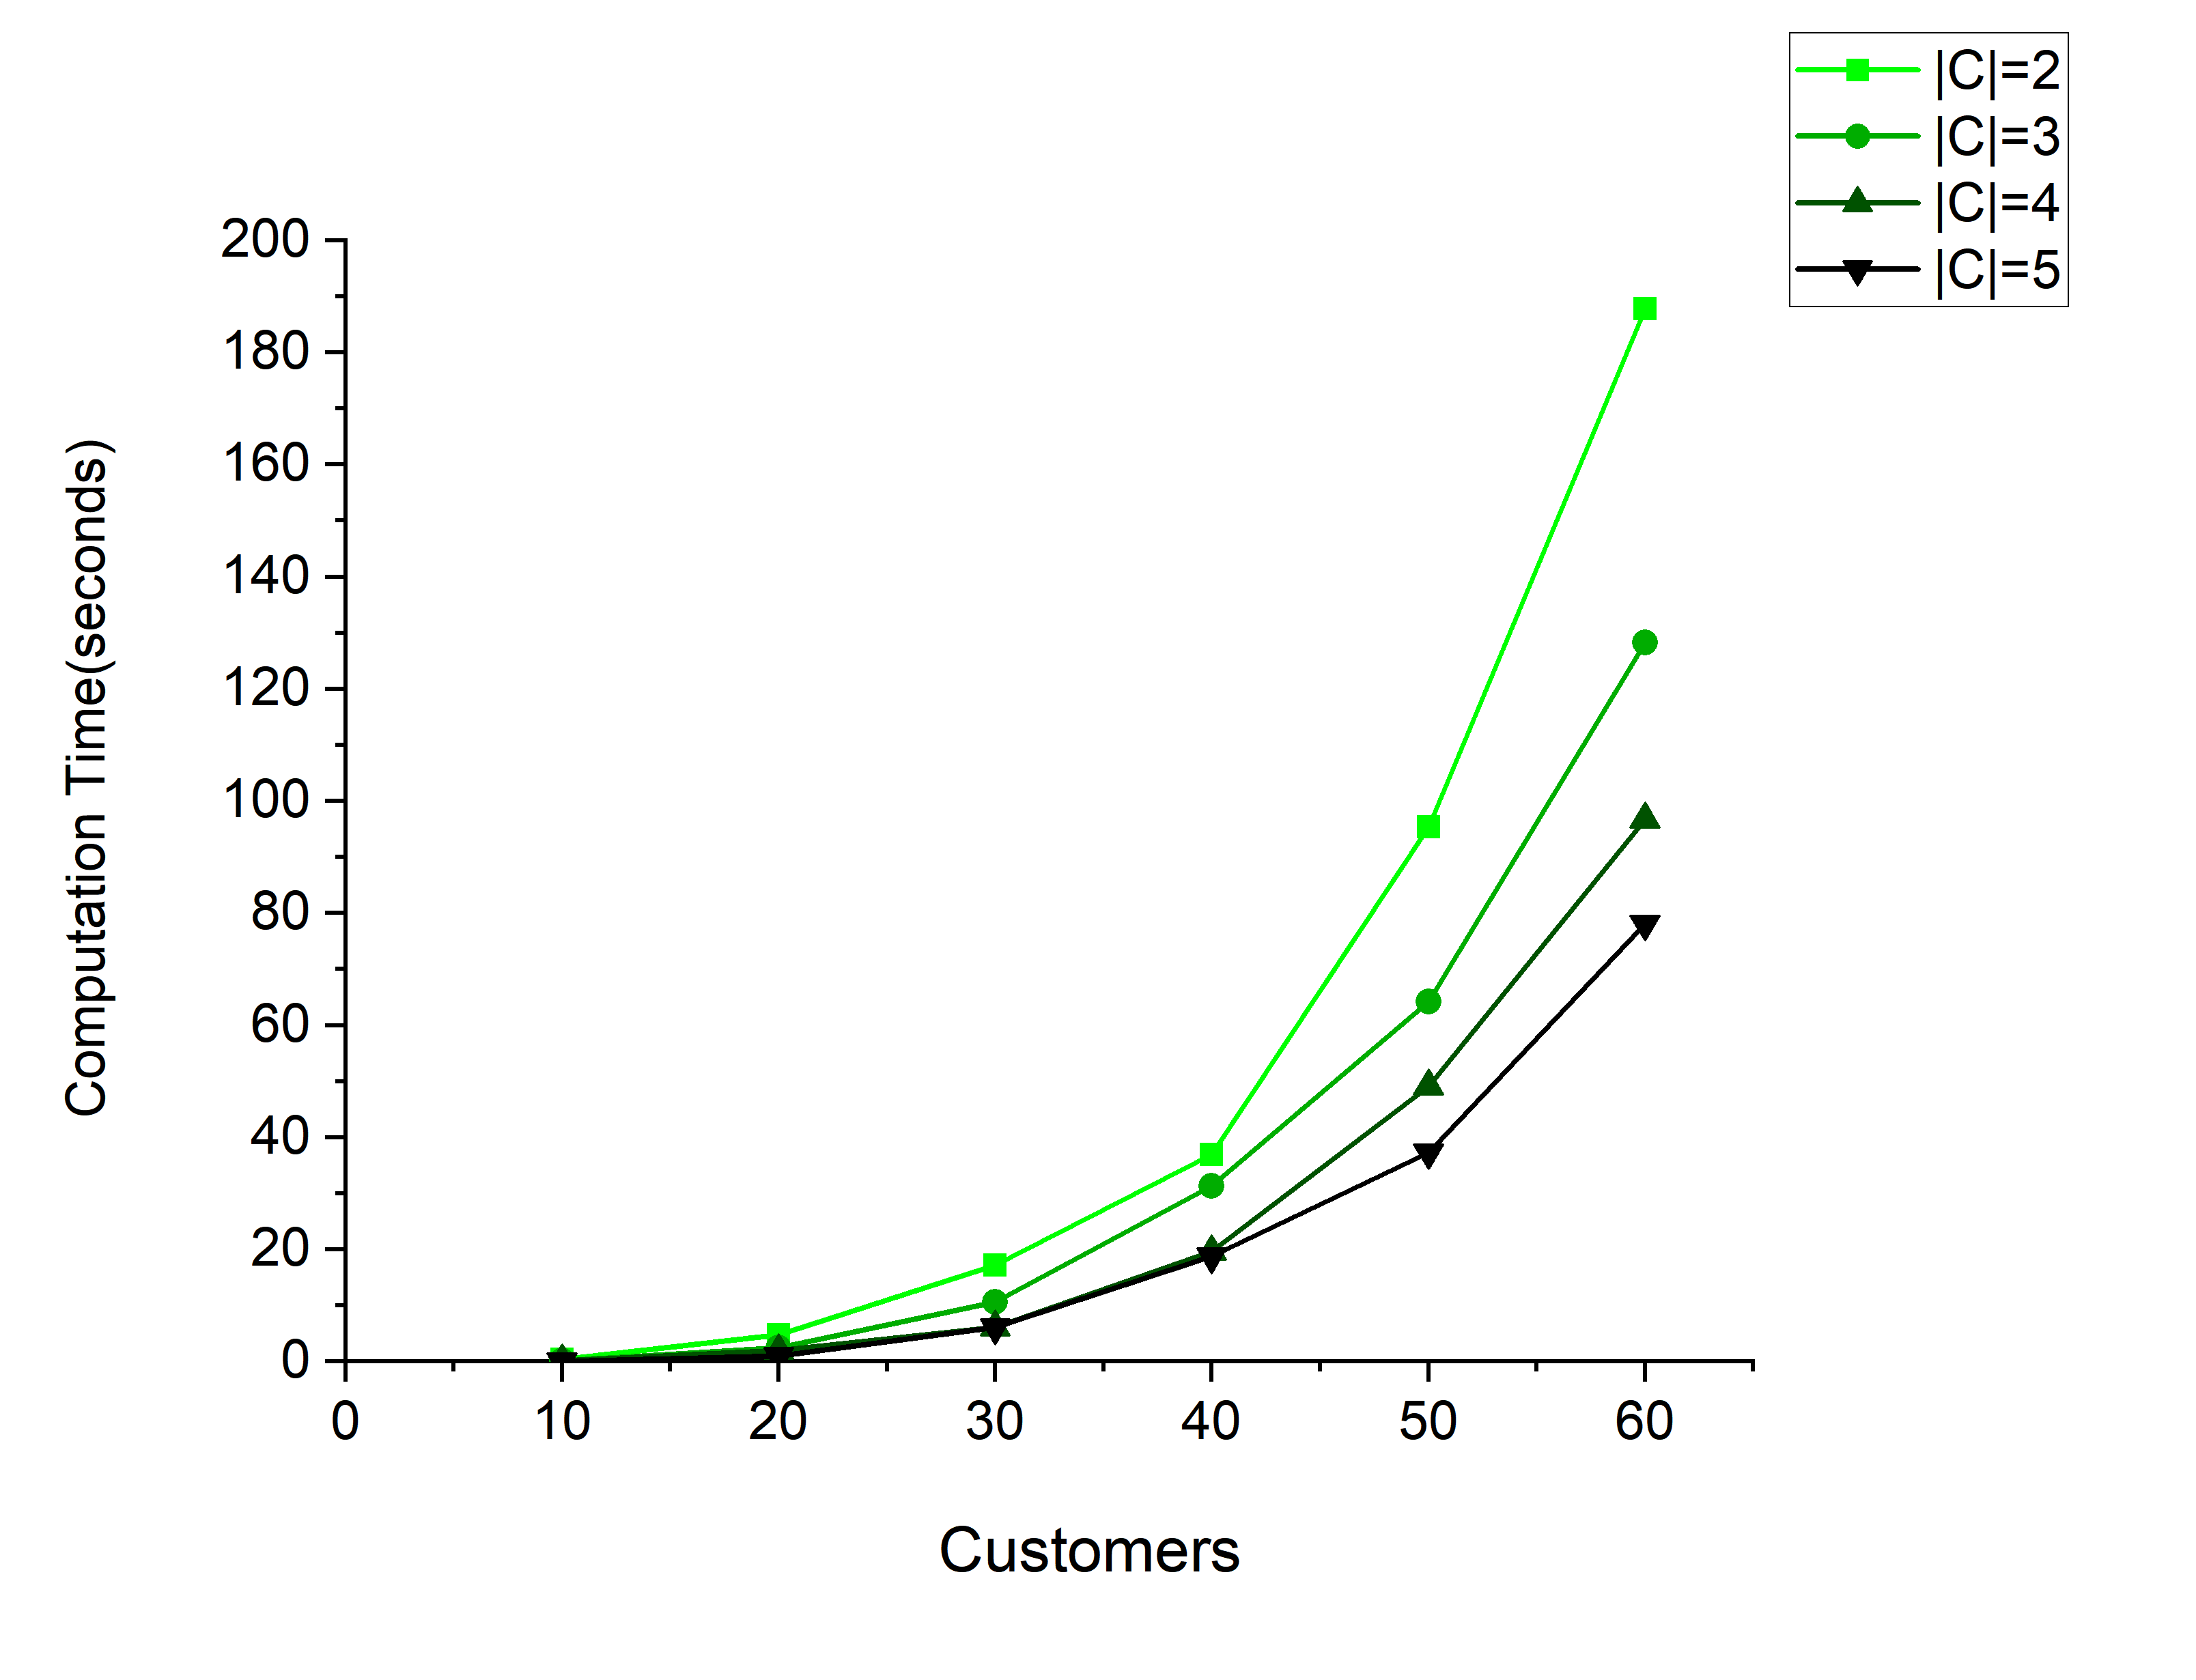
\includegraphics[width=\textwidth]{comp_alns.png}
%      \caption{Number of vehicle compartments}\label{fig:comp_alns}
%     \end{subfigure}
    
%     \begin{subfigure}[b]{0.2\textwidth}
%     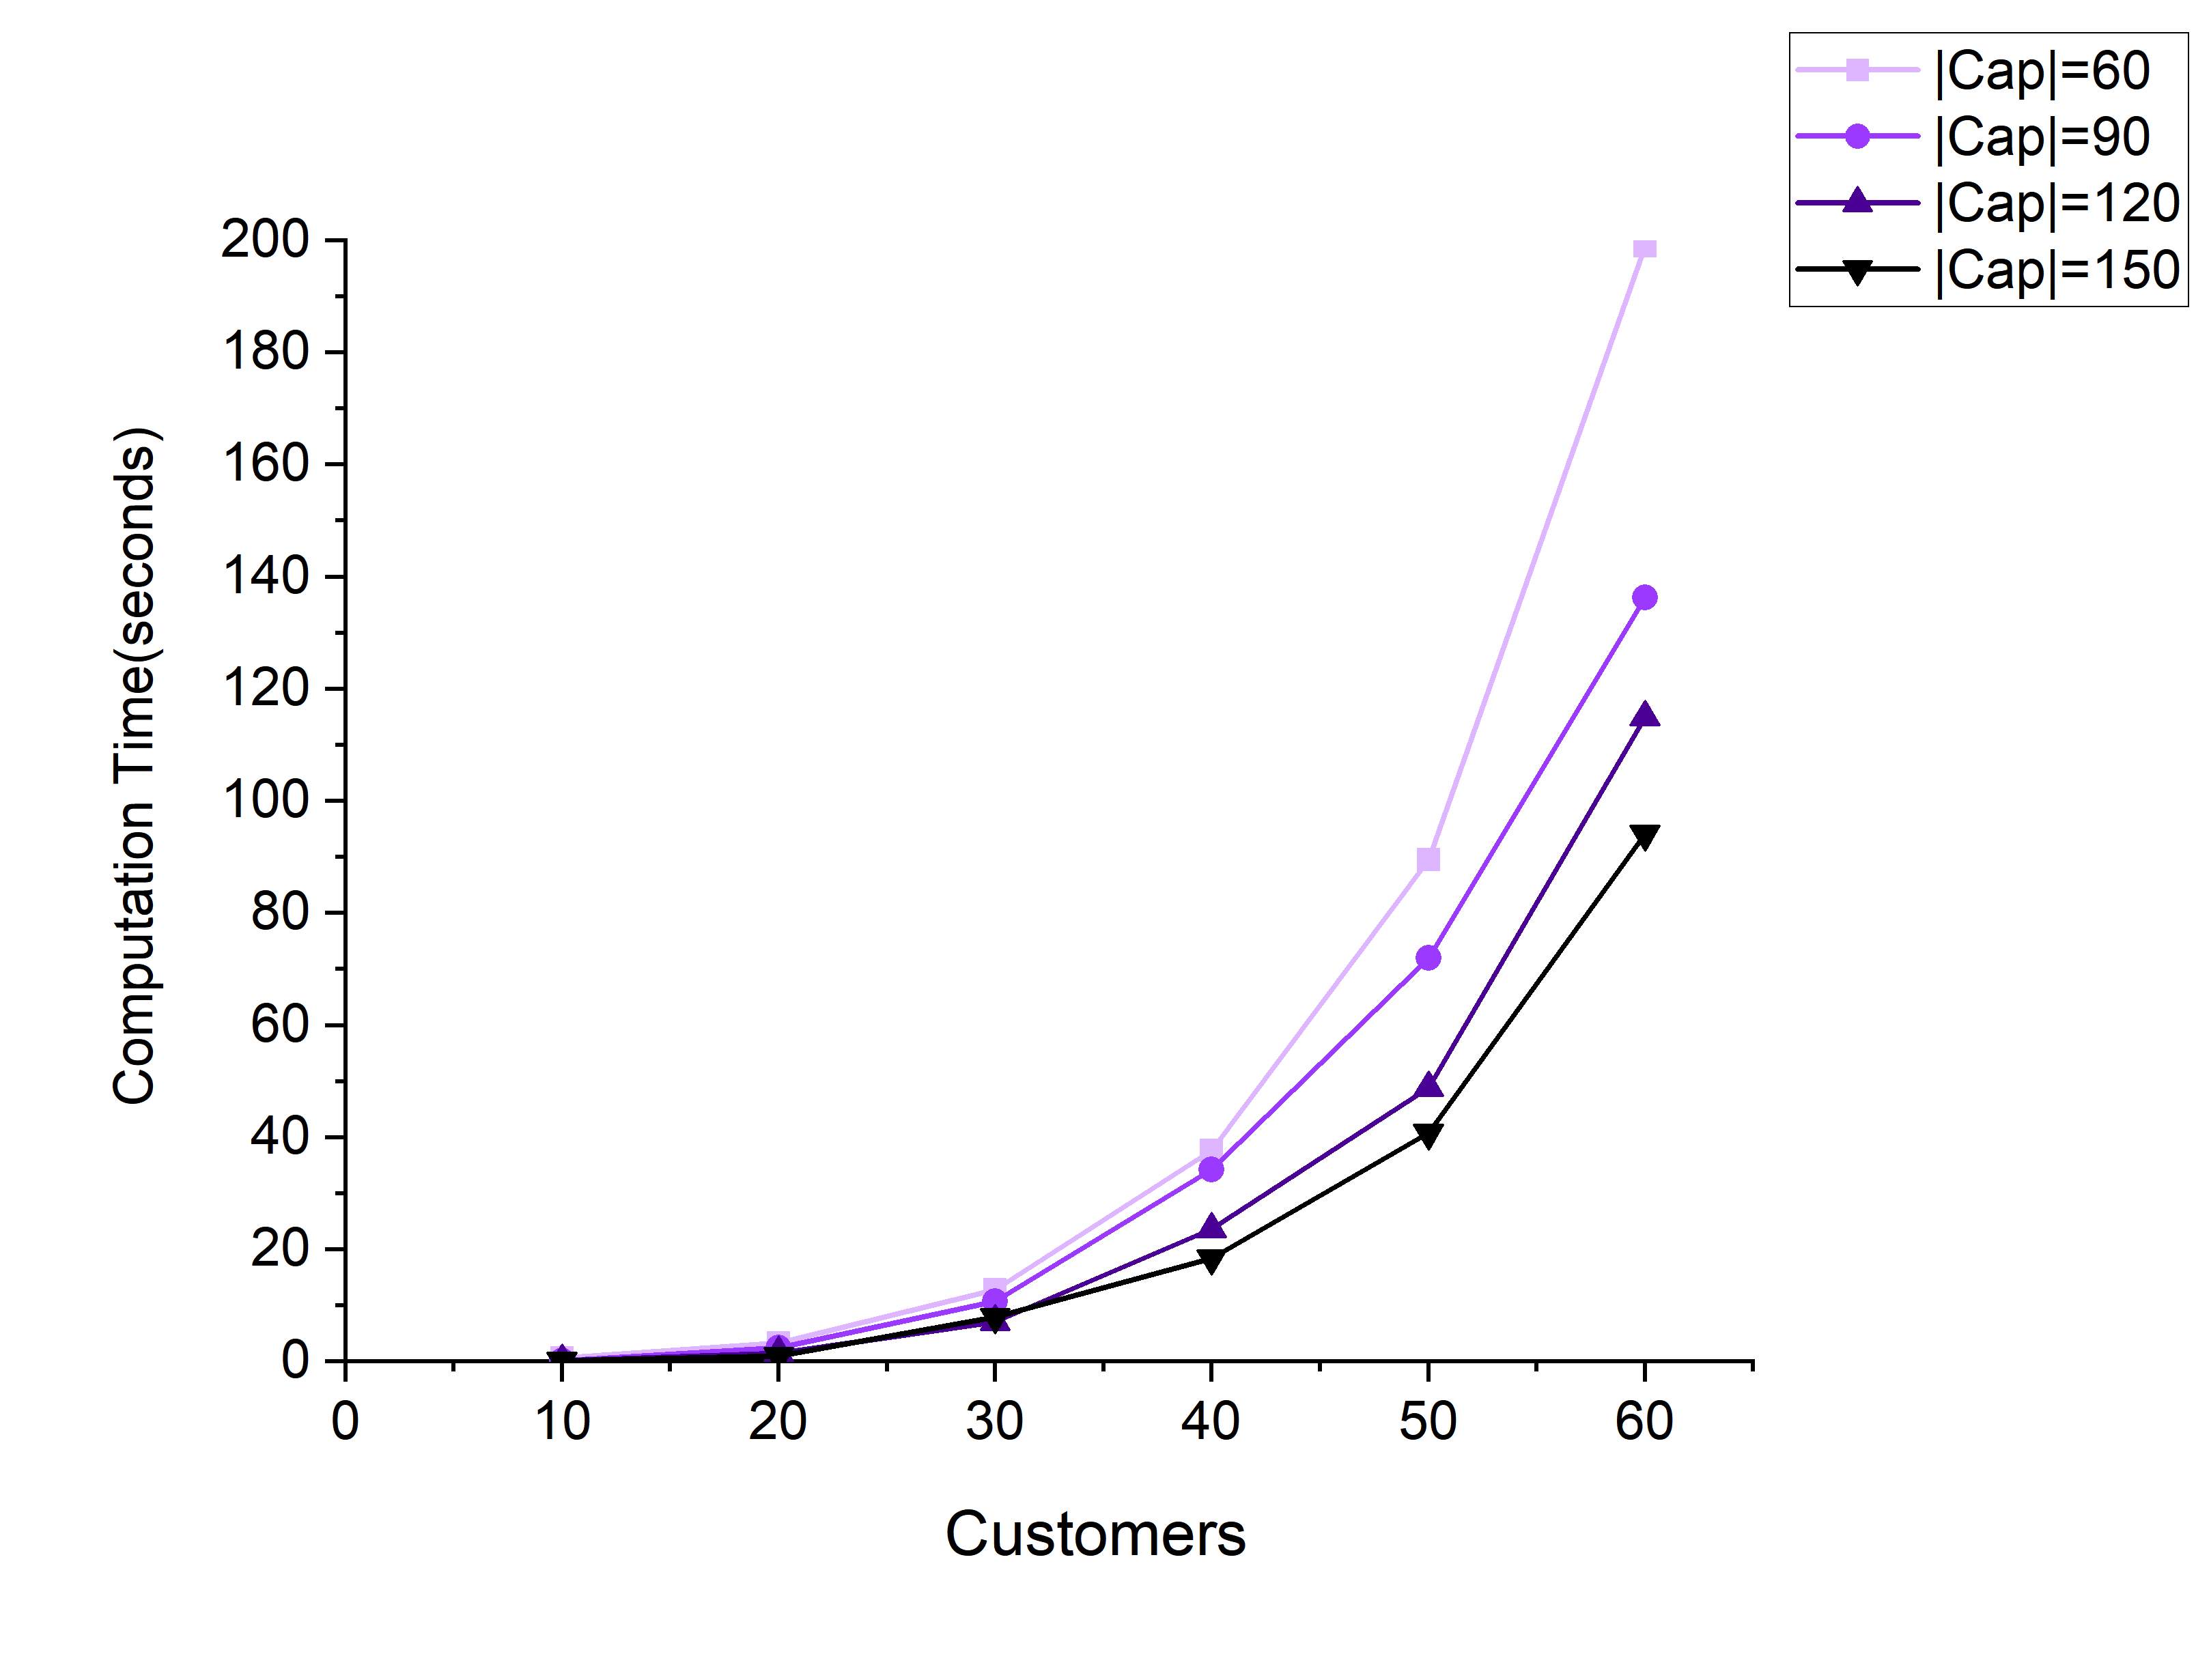
\includegraphics[width=\textwidth]{capa_alns.png}
%       \caption{Compartment capacity}\label{fig:capa_alns}
%     \end{subfigure}
%     \begin{subfigure}[b]{0.2\textwidth}
%     \qquad
%     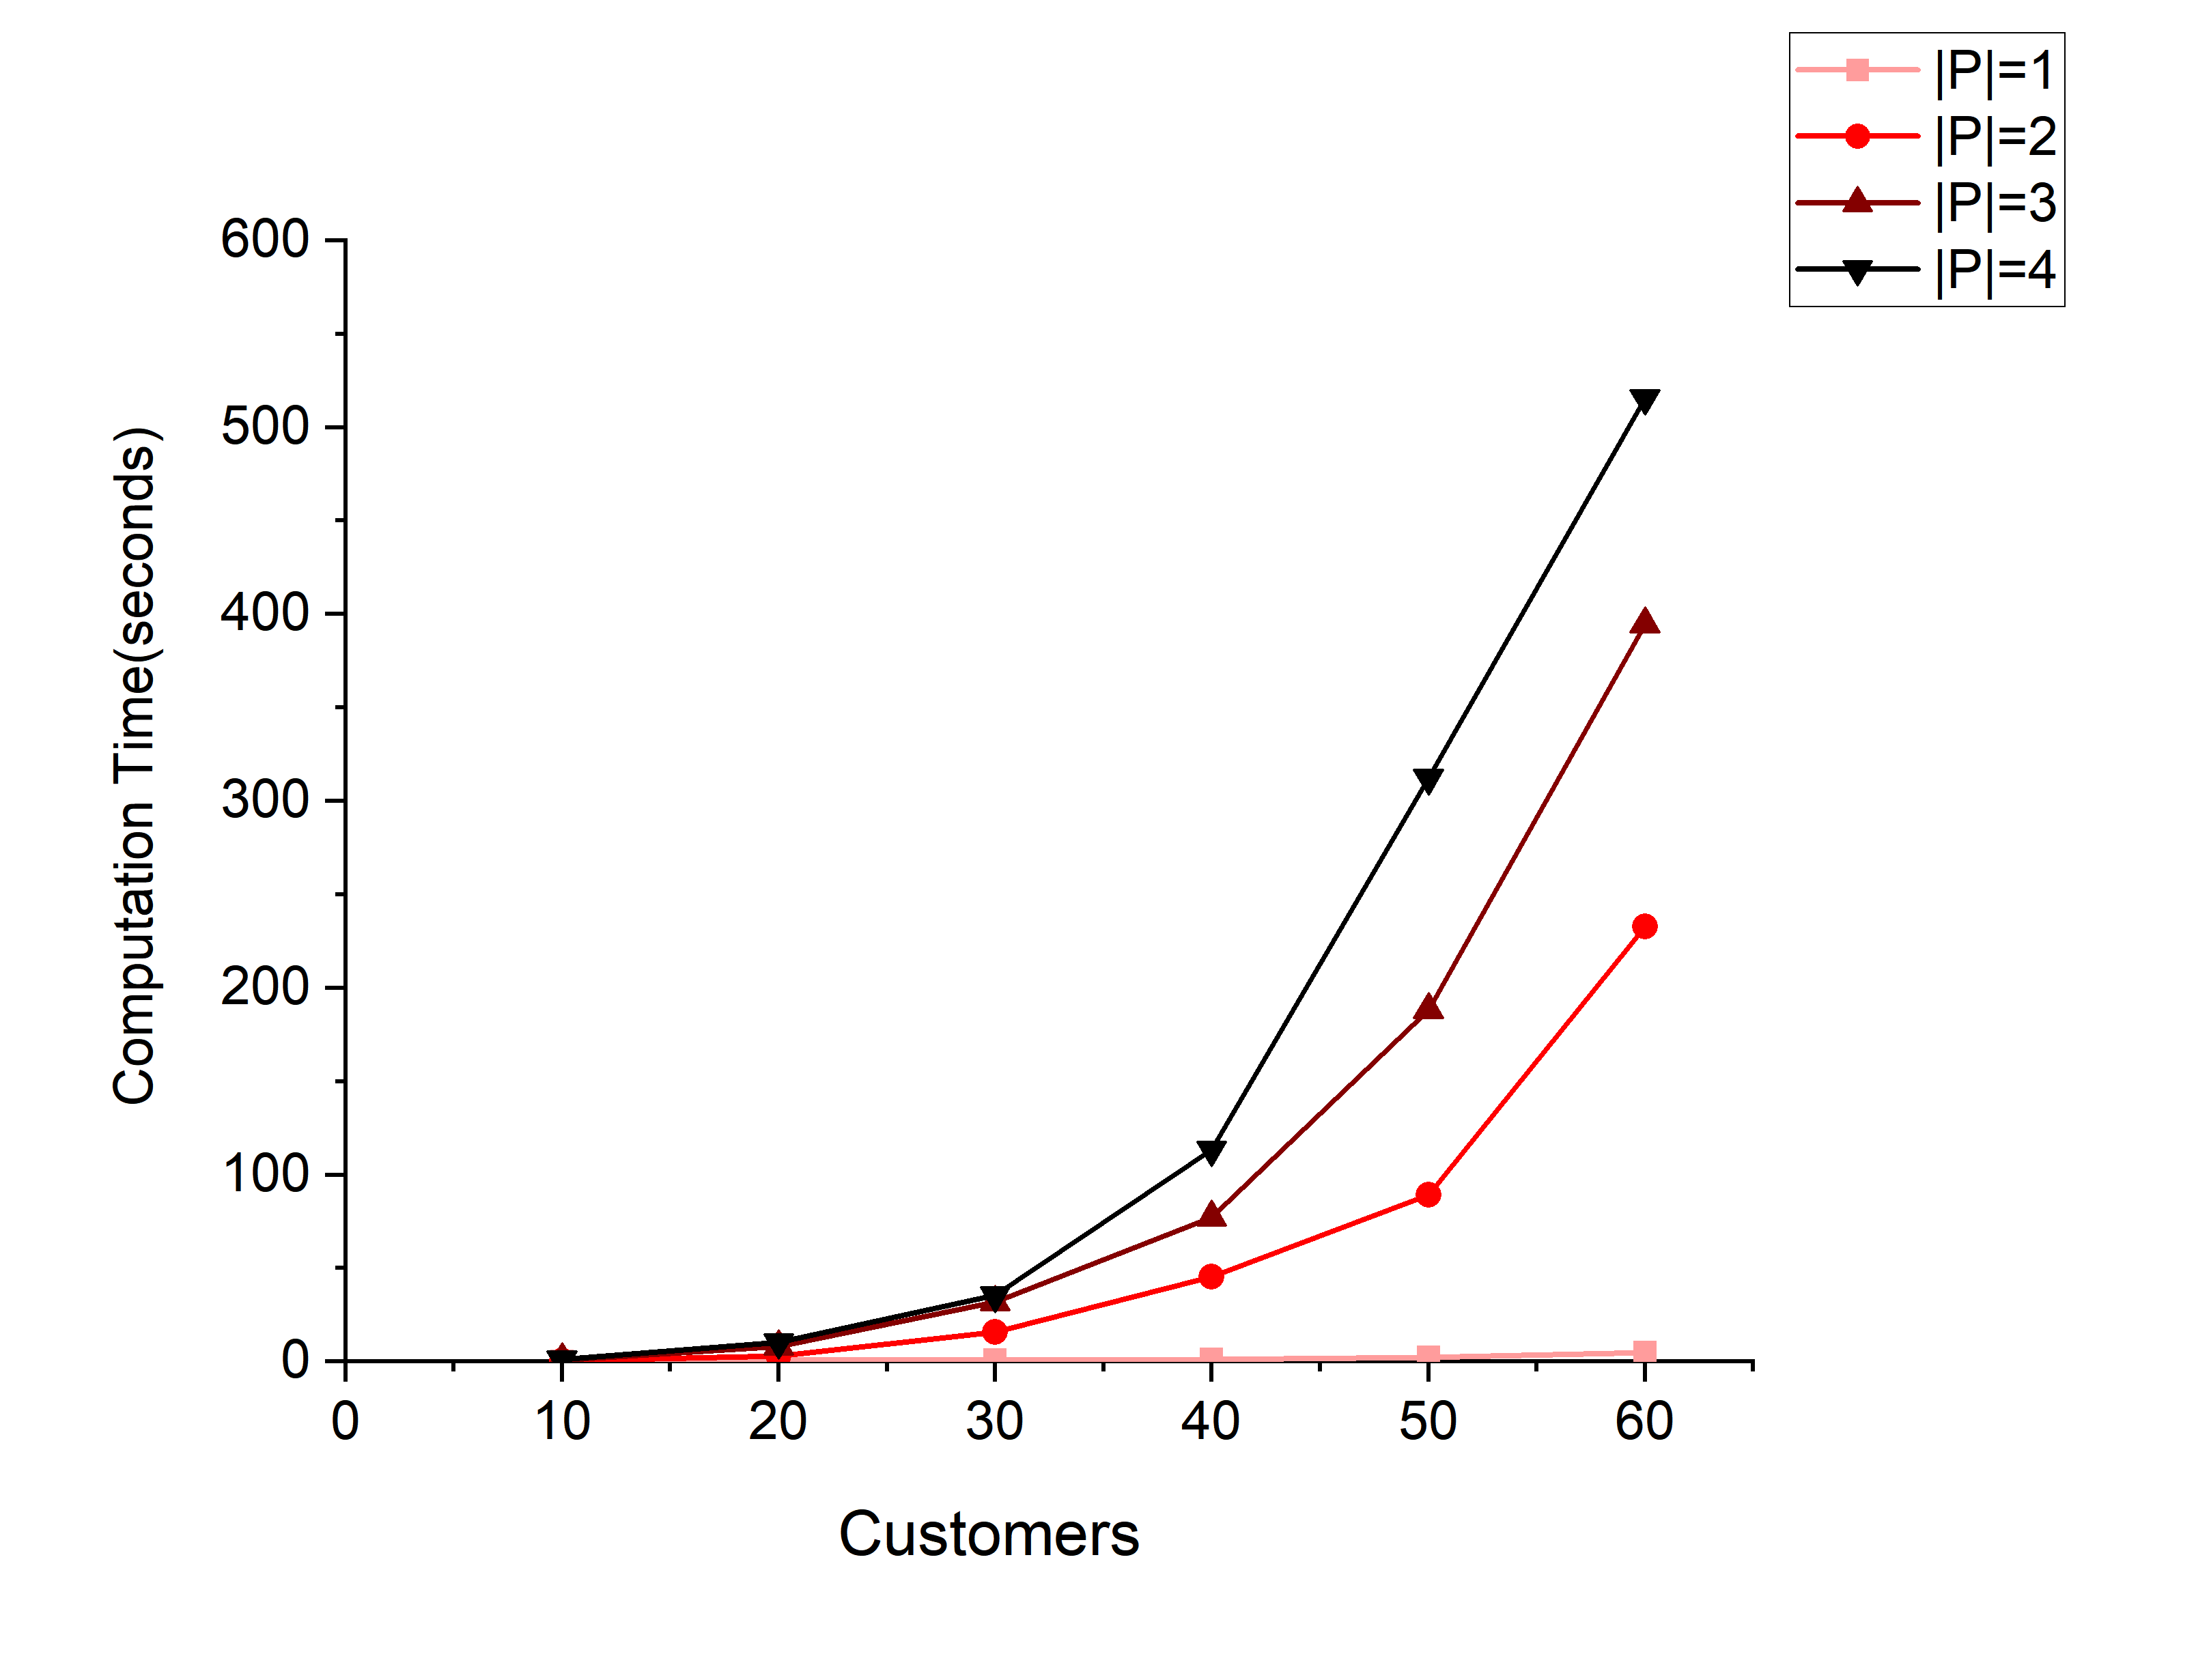
\includegraphics[width=\textwidth]{prod_alns.png}
%       \caption{Number of products}\label{fig:prod_alns}
%     \end{subfigure}
%     \caption{Impact of instance features on average ALNS computation time.}
%     \label{fig:s-pricing}
% \end{figure}

%\subsubsection{influence of the budget}\label{sec:exp-budget}
%In general, the business manager will decide the budget through their experience. However, it is hard to measure the effectiveness of the budget setup made by personal experience. Therefore, in this section, we provide an analytical tool to facilitate the recommendation of the budget setup. We consider the difference between the single-stage pricing and the unified pricing mechanism as the effectiveness of the single-stage pricing. Interesting to observe is that, as the budget increases, the effectiveness increases first and then decreases. We discover the highest point is reached when the budget is around xx. We can suggest a reasonable range of the budget from xx to xx. Therefore, this phenomenon verifies the effectiveness of our single-stage pricing method.

% \begin{figure}[tb]
%     \centering
%     \begin{subfigure}[b]{0.2\textwidth}
%     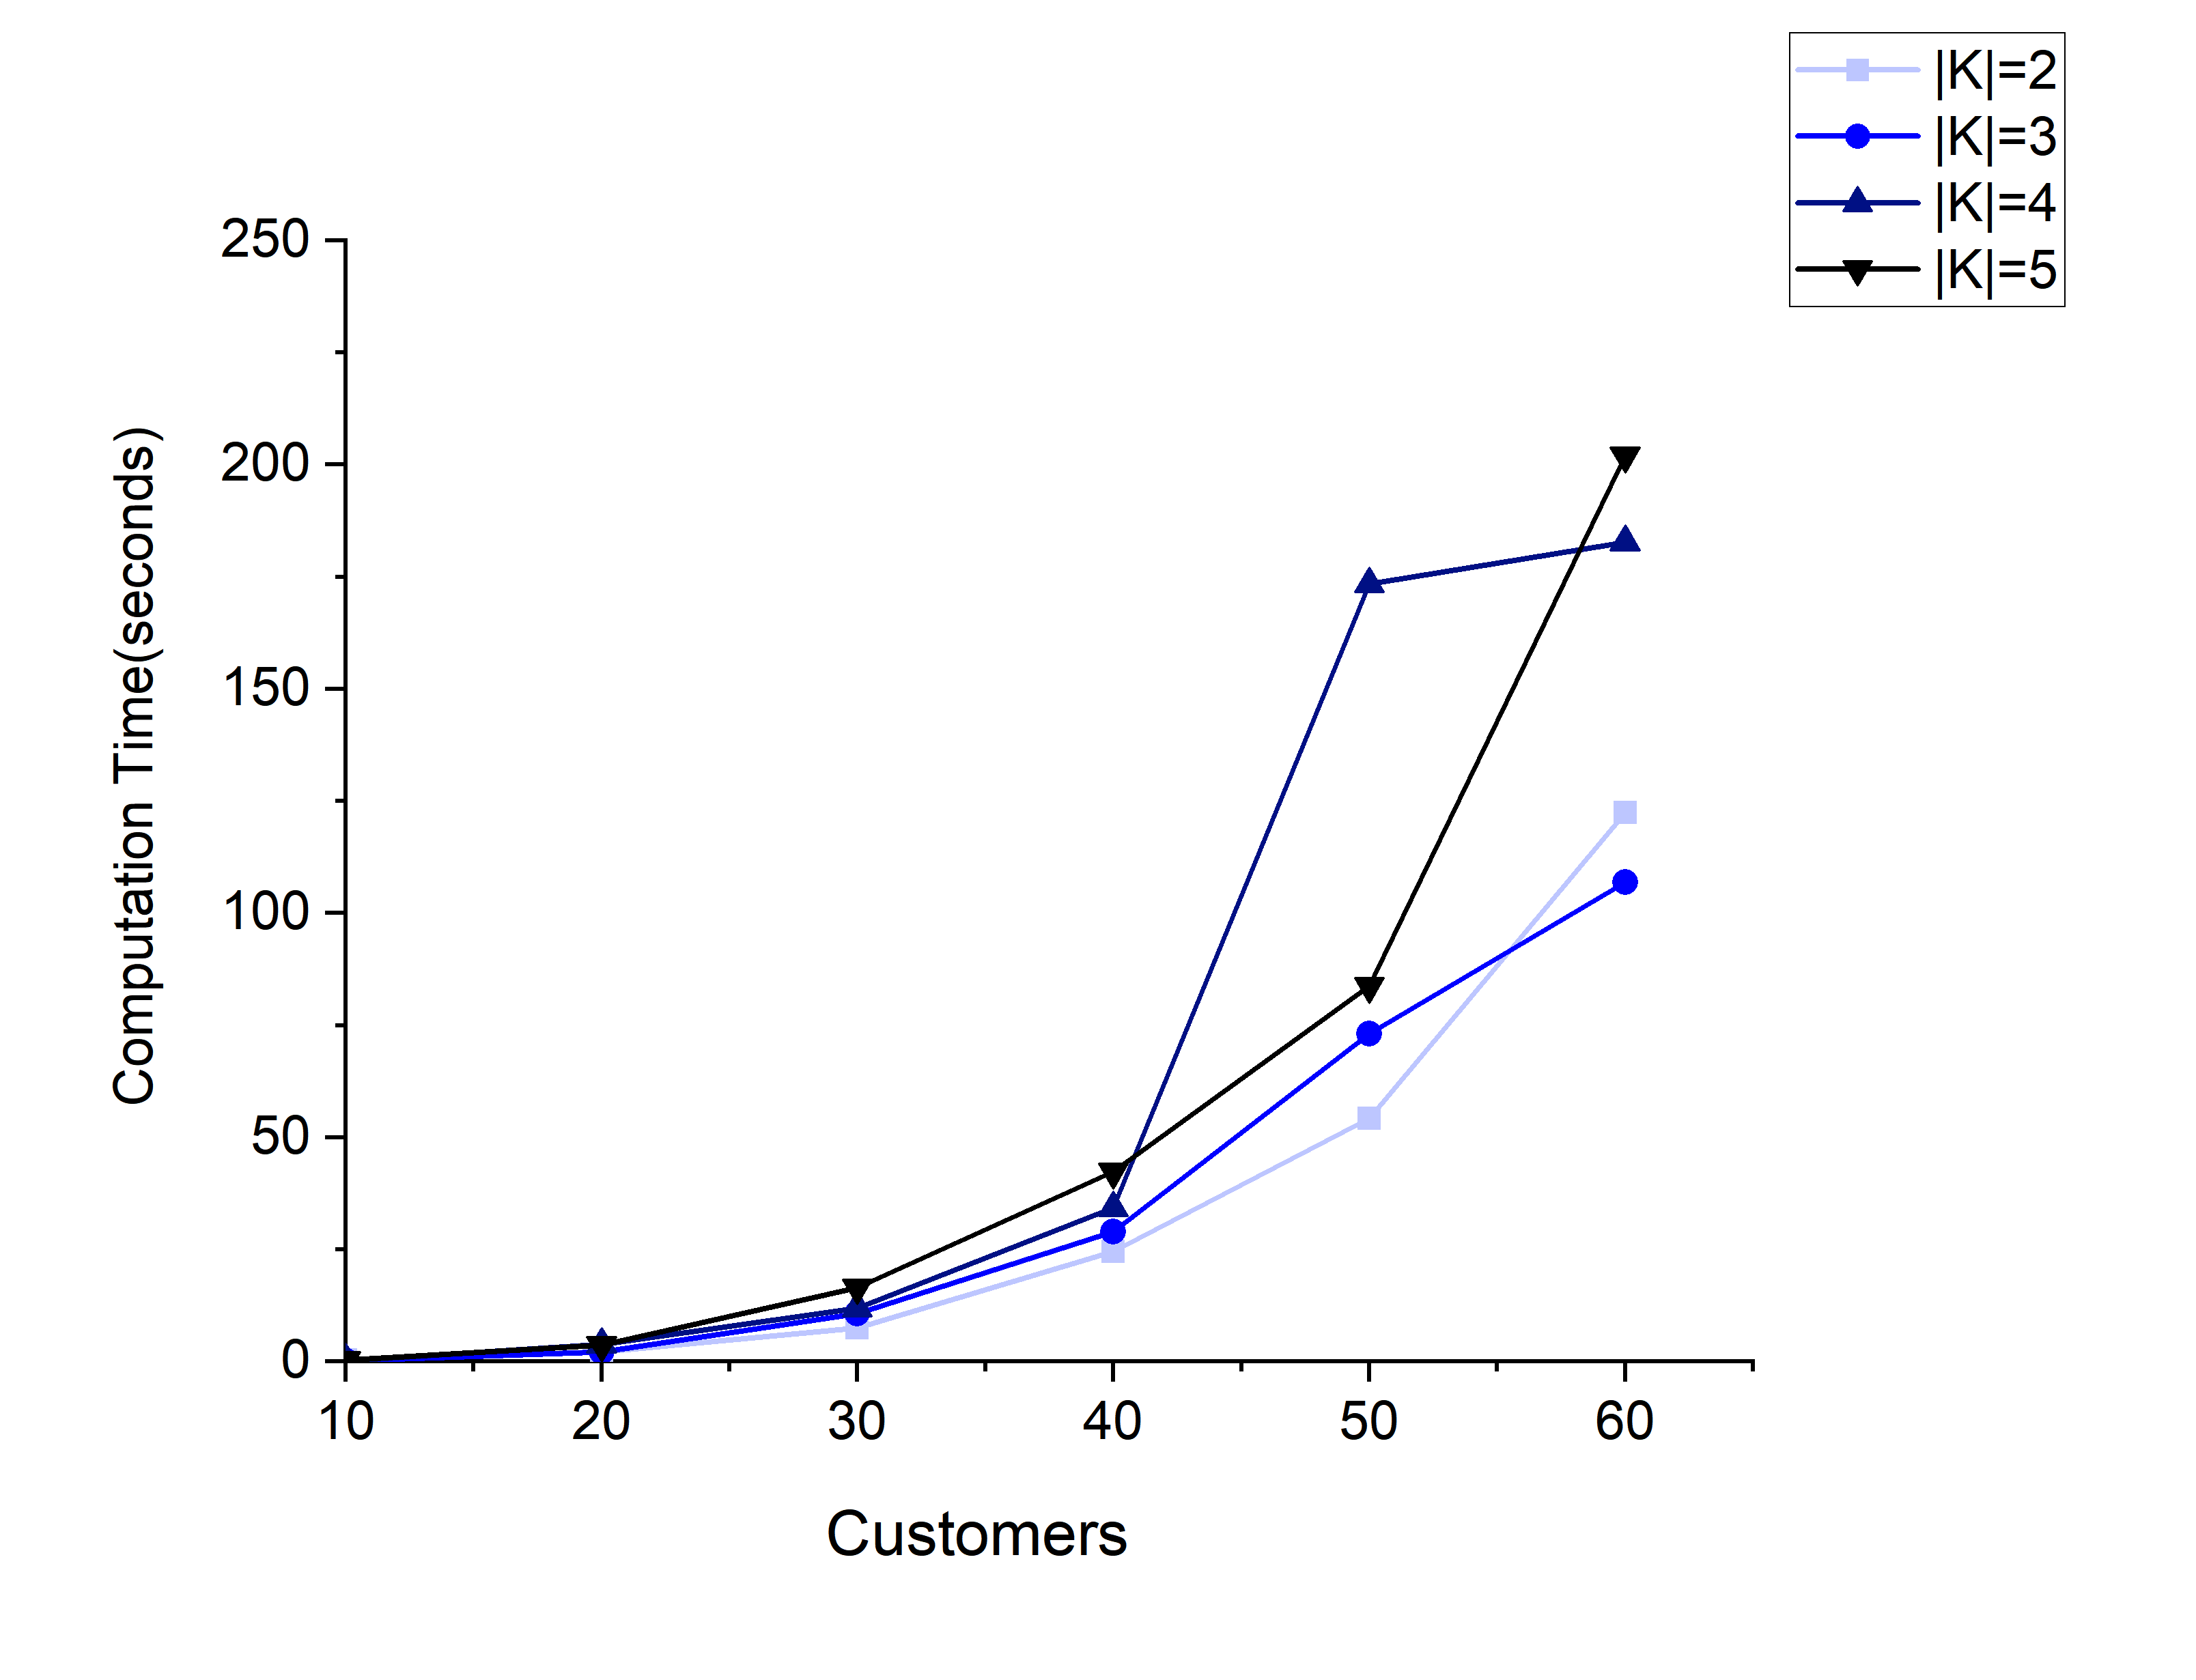
\includegraphics[width=\textwidth]{vehi_alns.png}
  
%         \caption{Number of vehicles}\label{fig:vehi_alns}
%     \end{subfigure}
%     \quad
%     \begin{subfigure}[b]{0.2\textwidth}
%     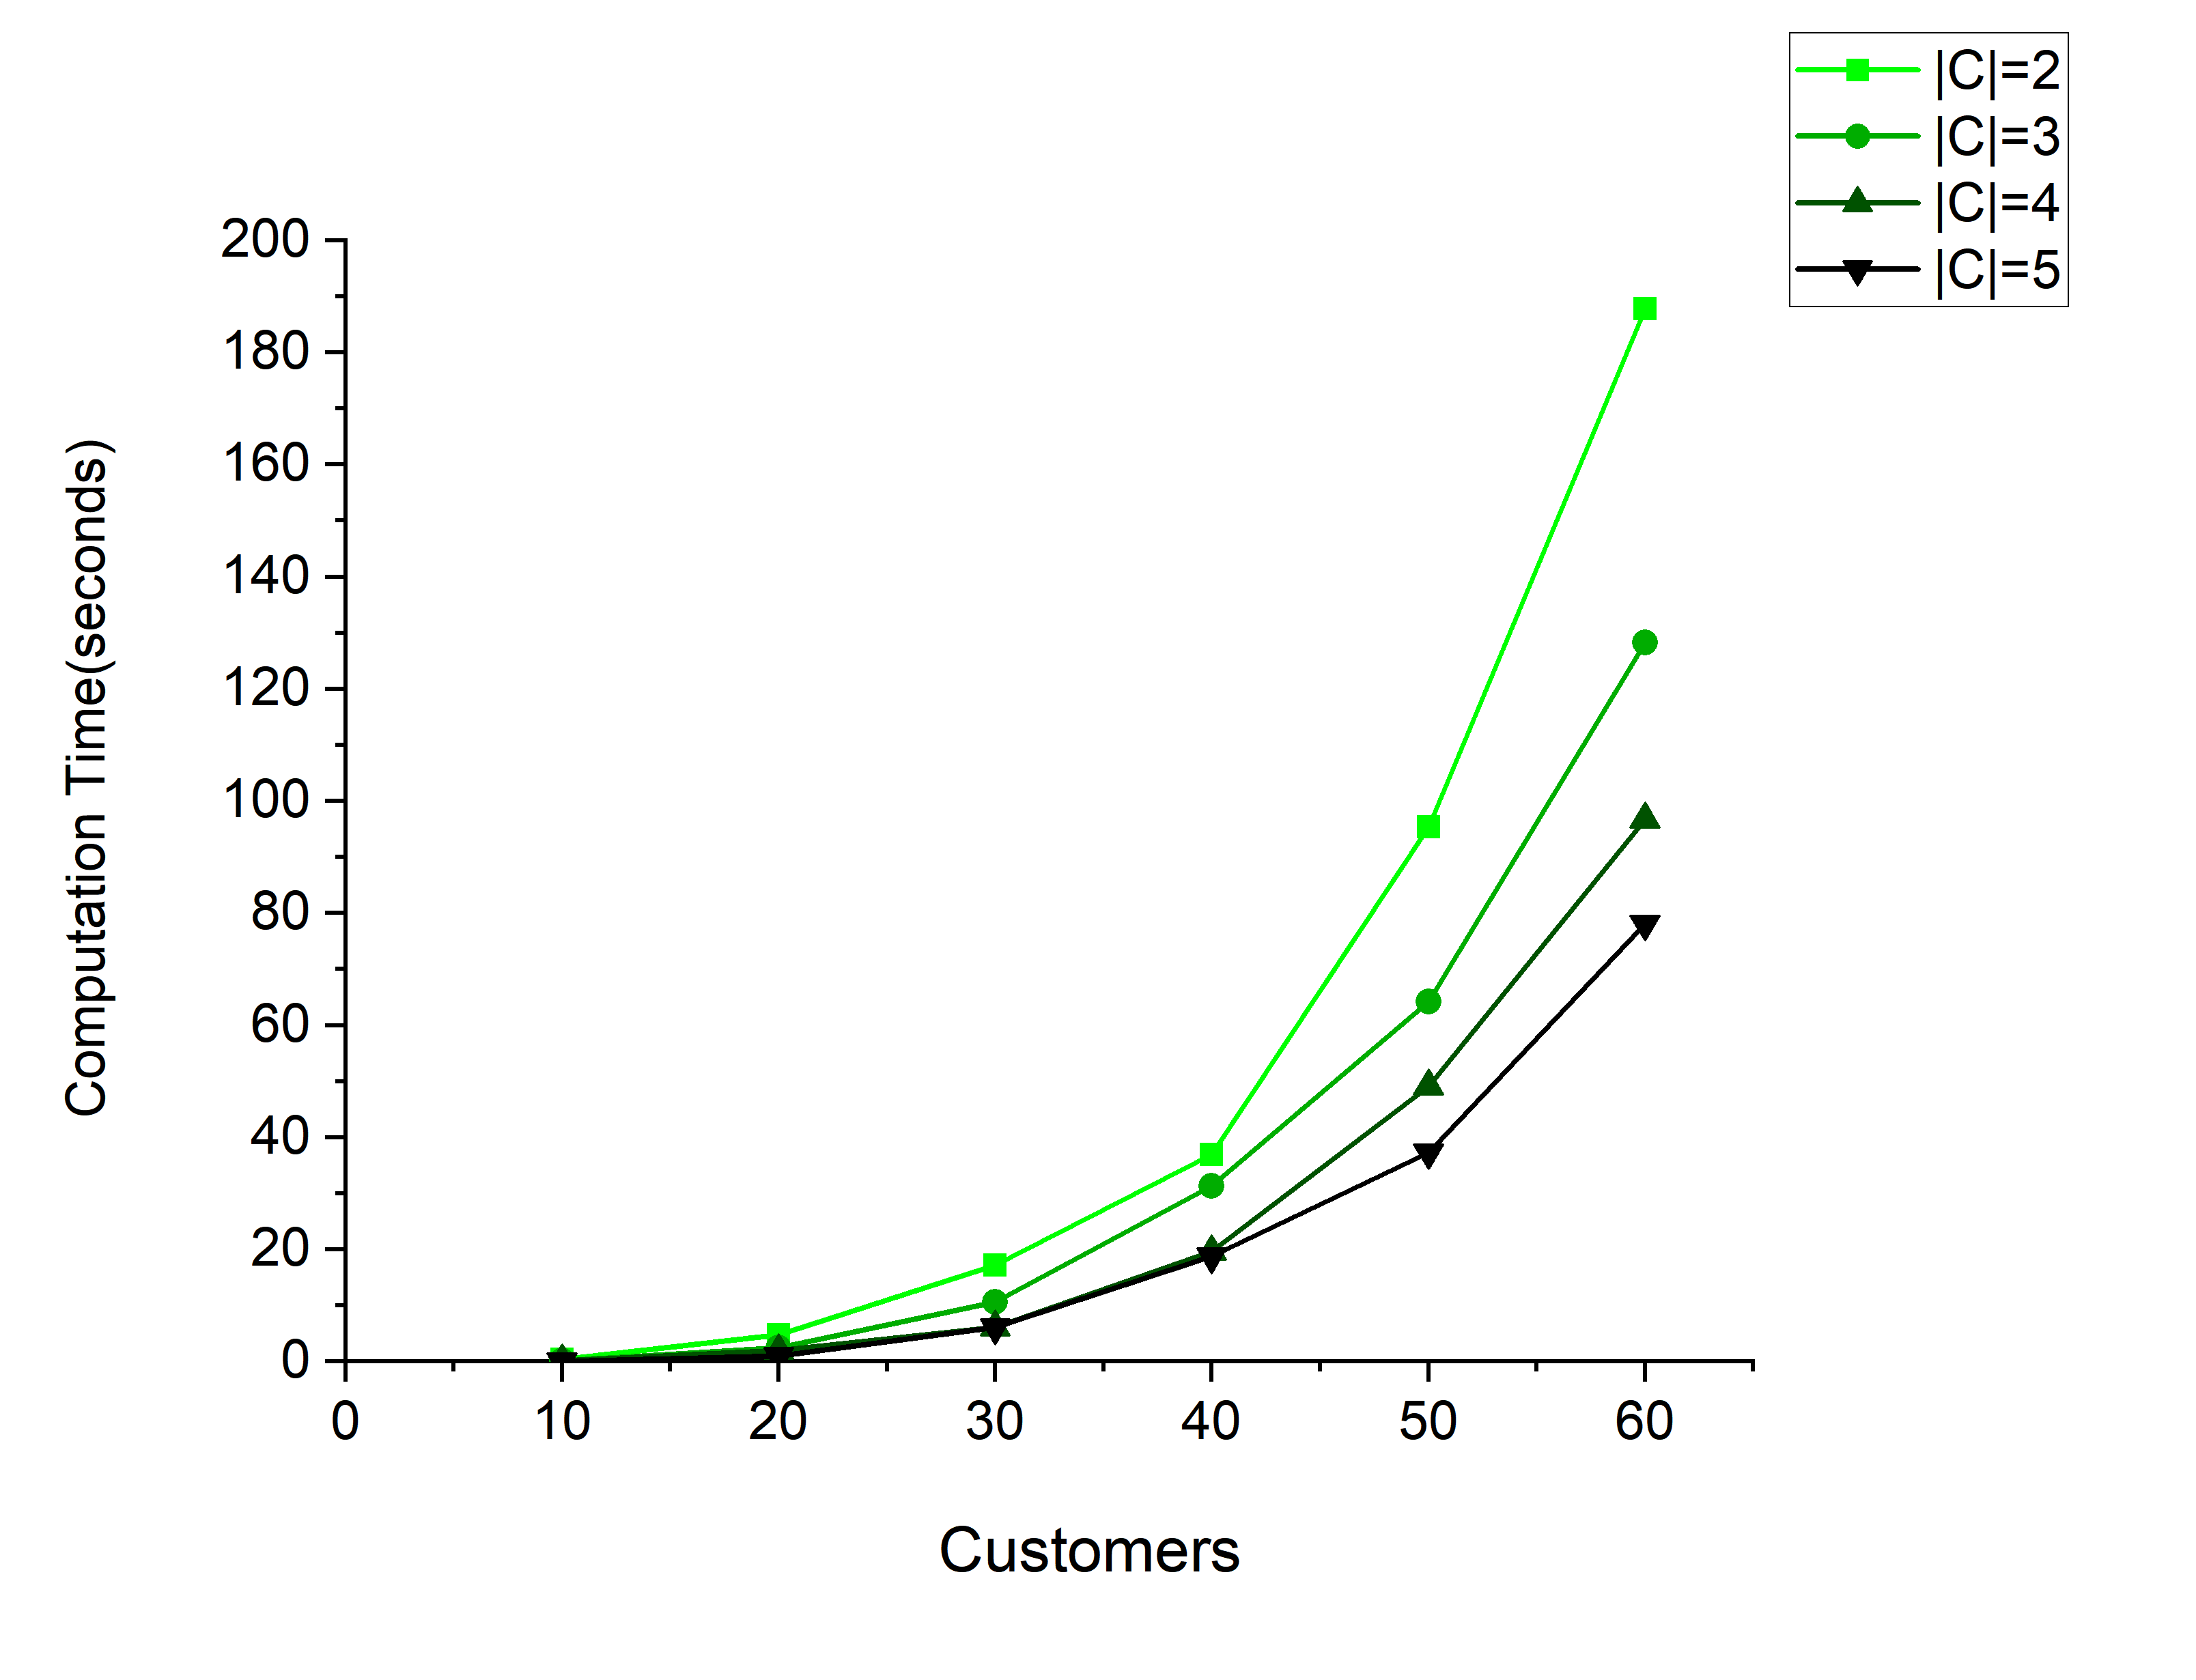
\includegraphics[width=\textwidth]{comp_alns.png}
%      \caption{Number of vehicle compartments}\label{fig:comp_alns}
%     \end{subfigure}
    
%     \begin{subfigure}[b]{0.2\textwidth}
%     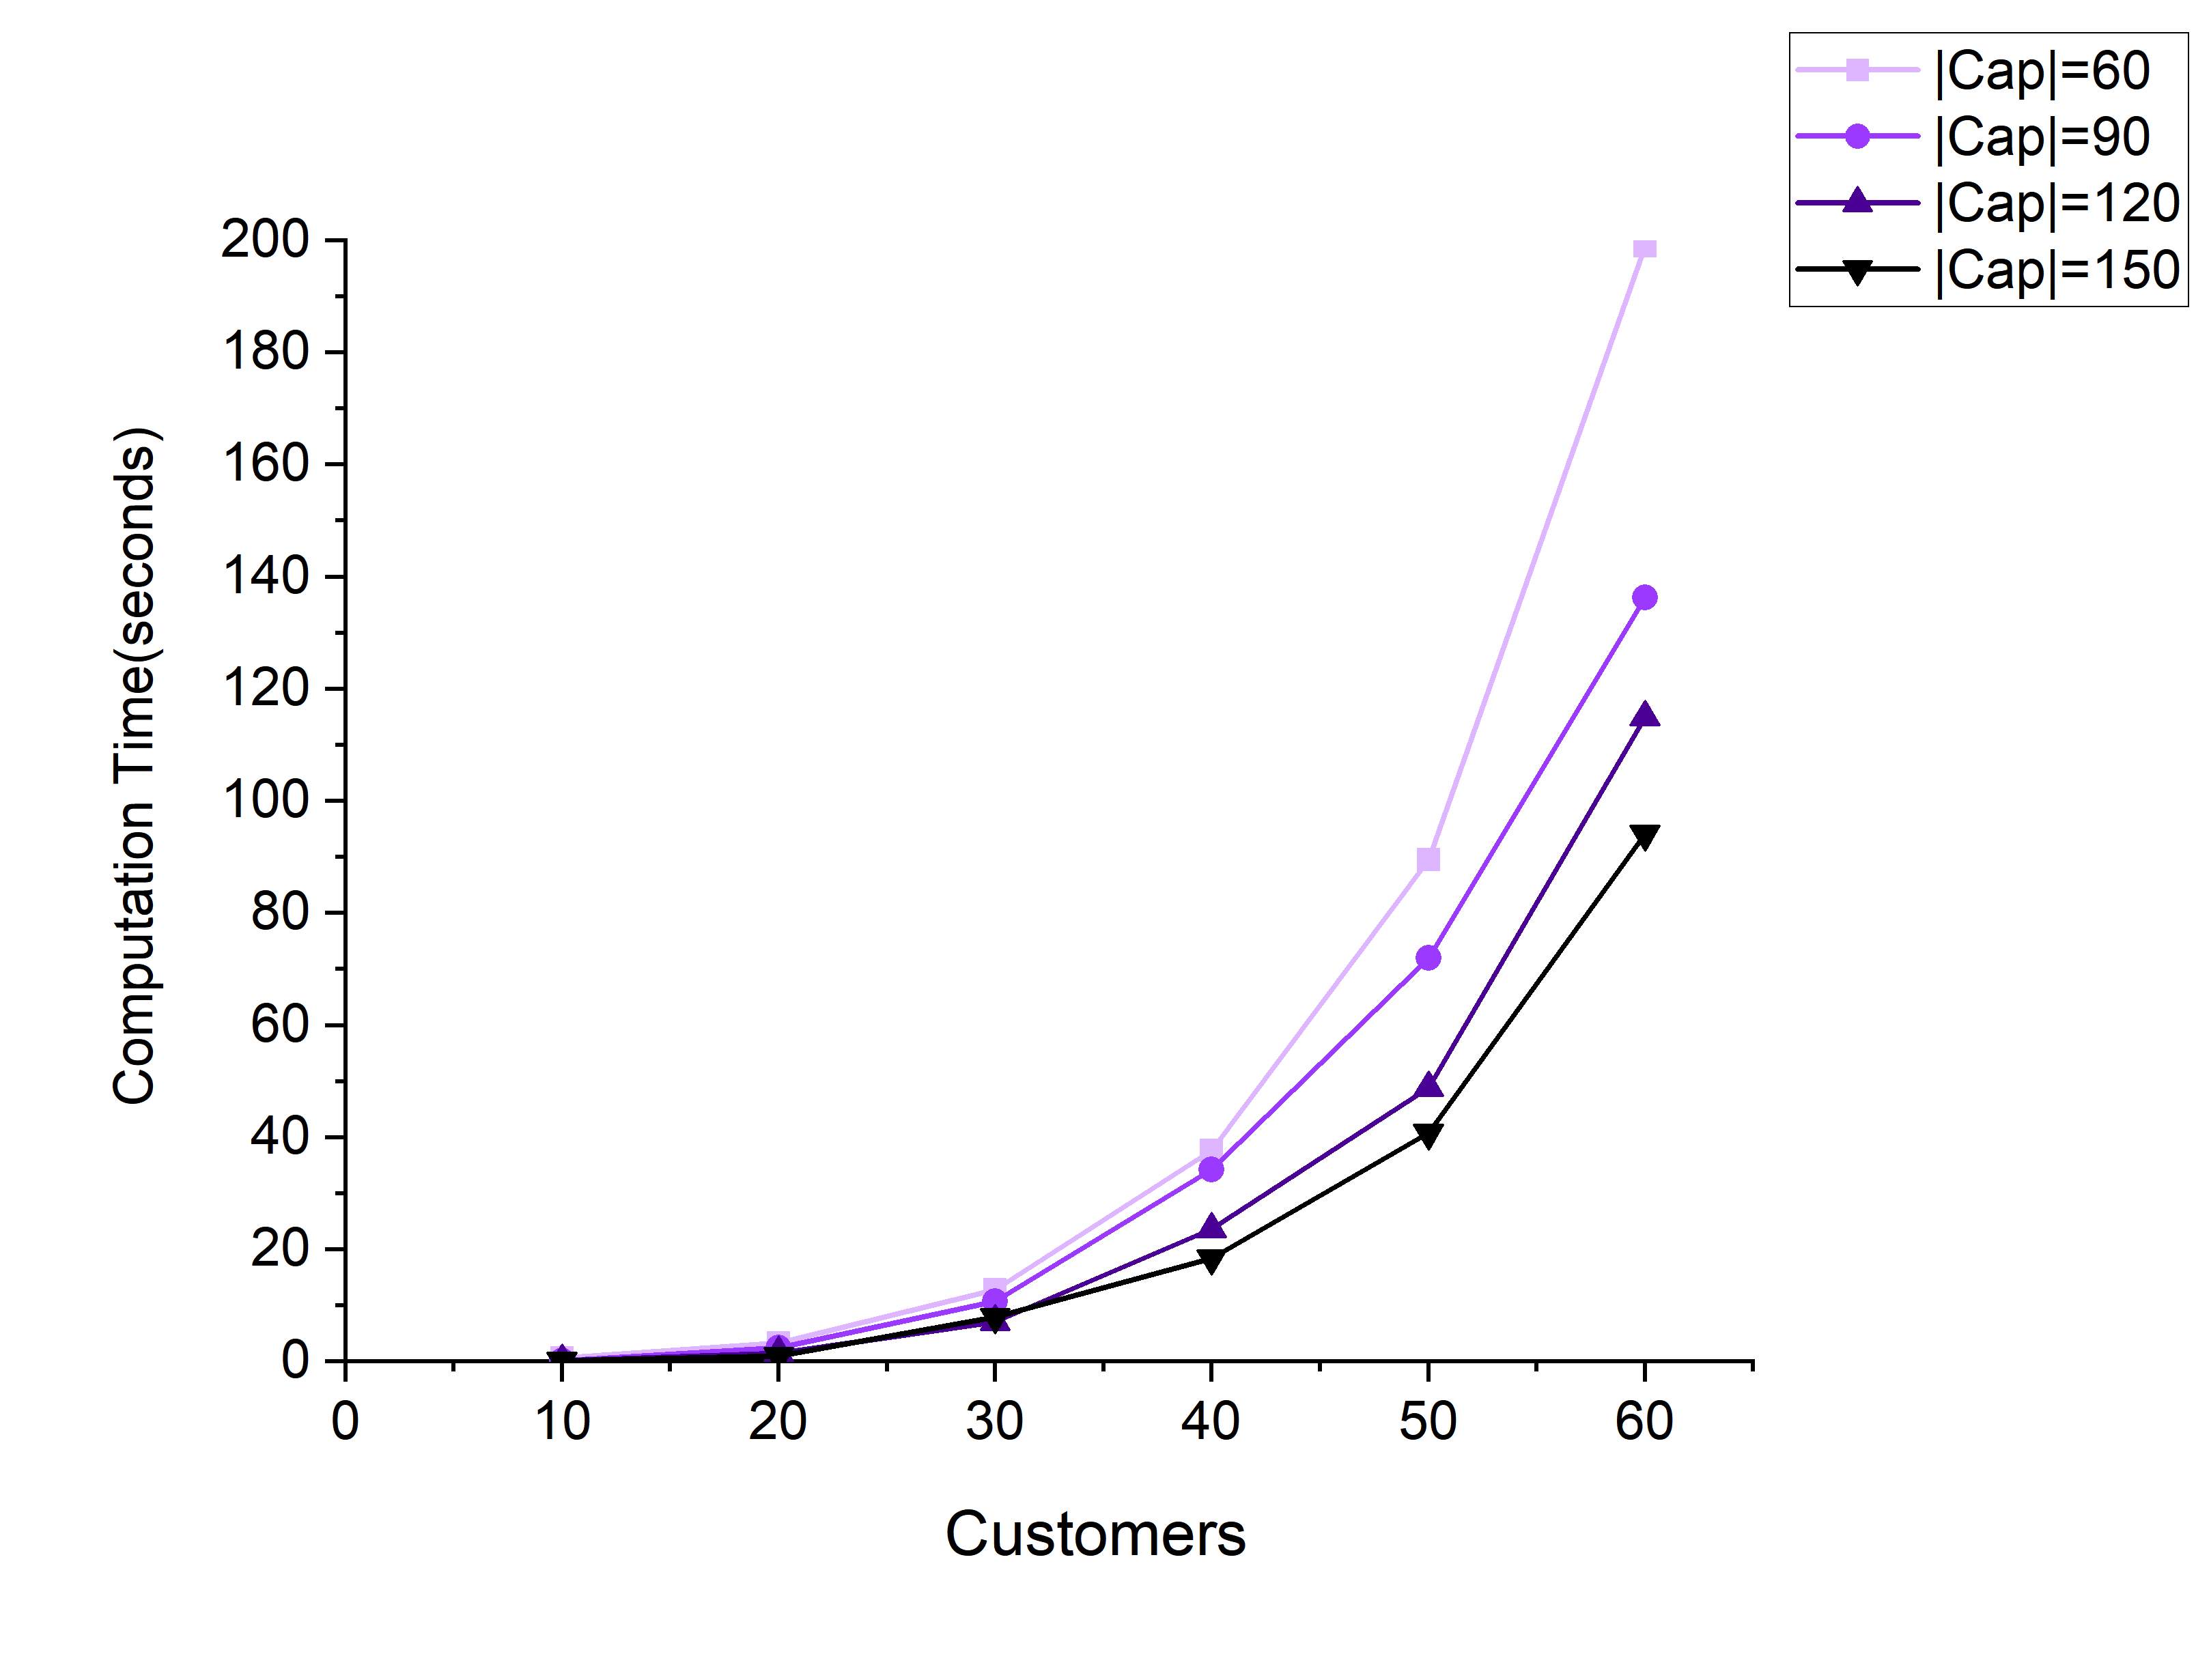
\includegraphics[width=\textwidth]{capa_alns.png}
%       \caption{Compartment capacity}\label{fig:capa_alns}
%     \end{subfigure}
%     \begin{subfigure}[b]{0.2\textwidth}
%     \qquad
%     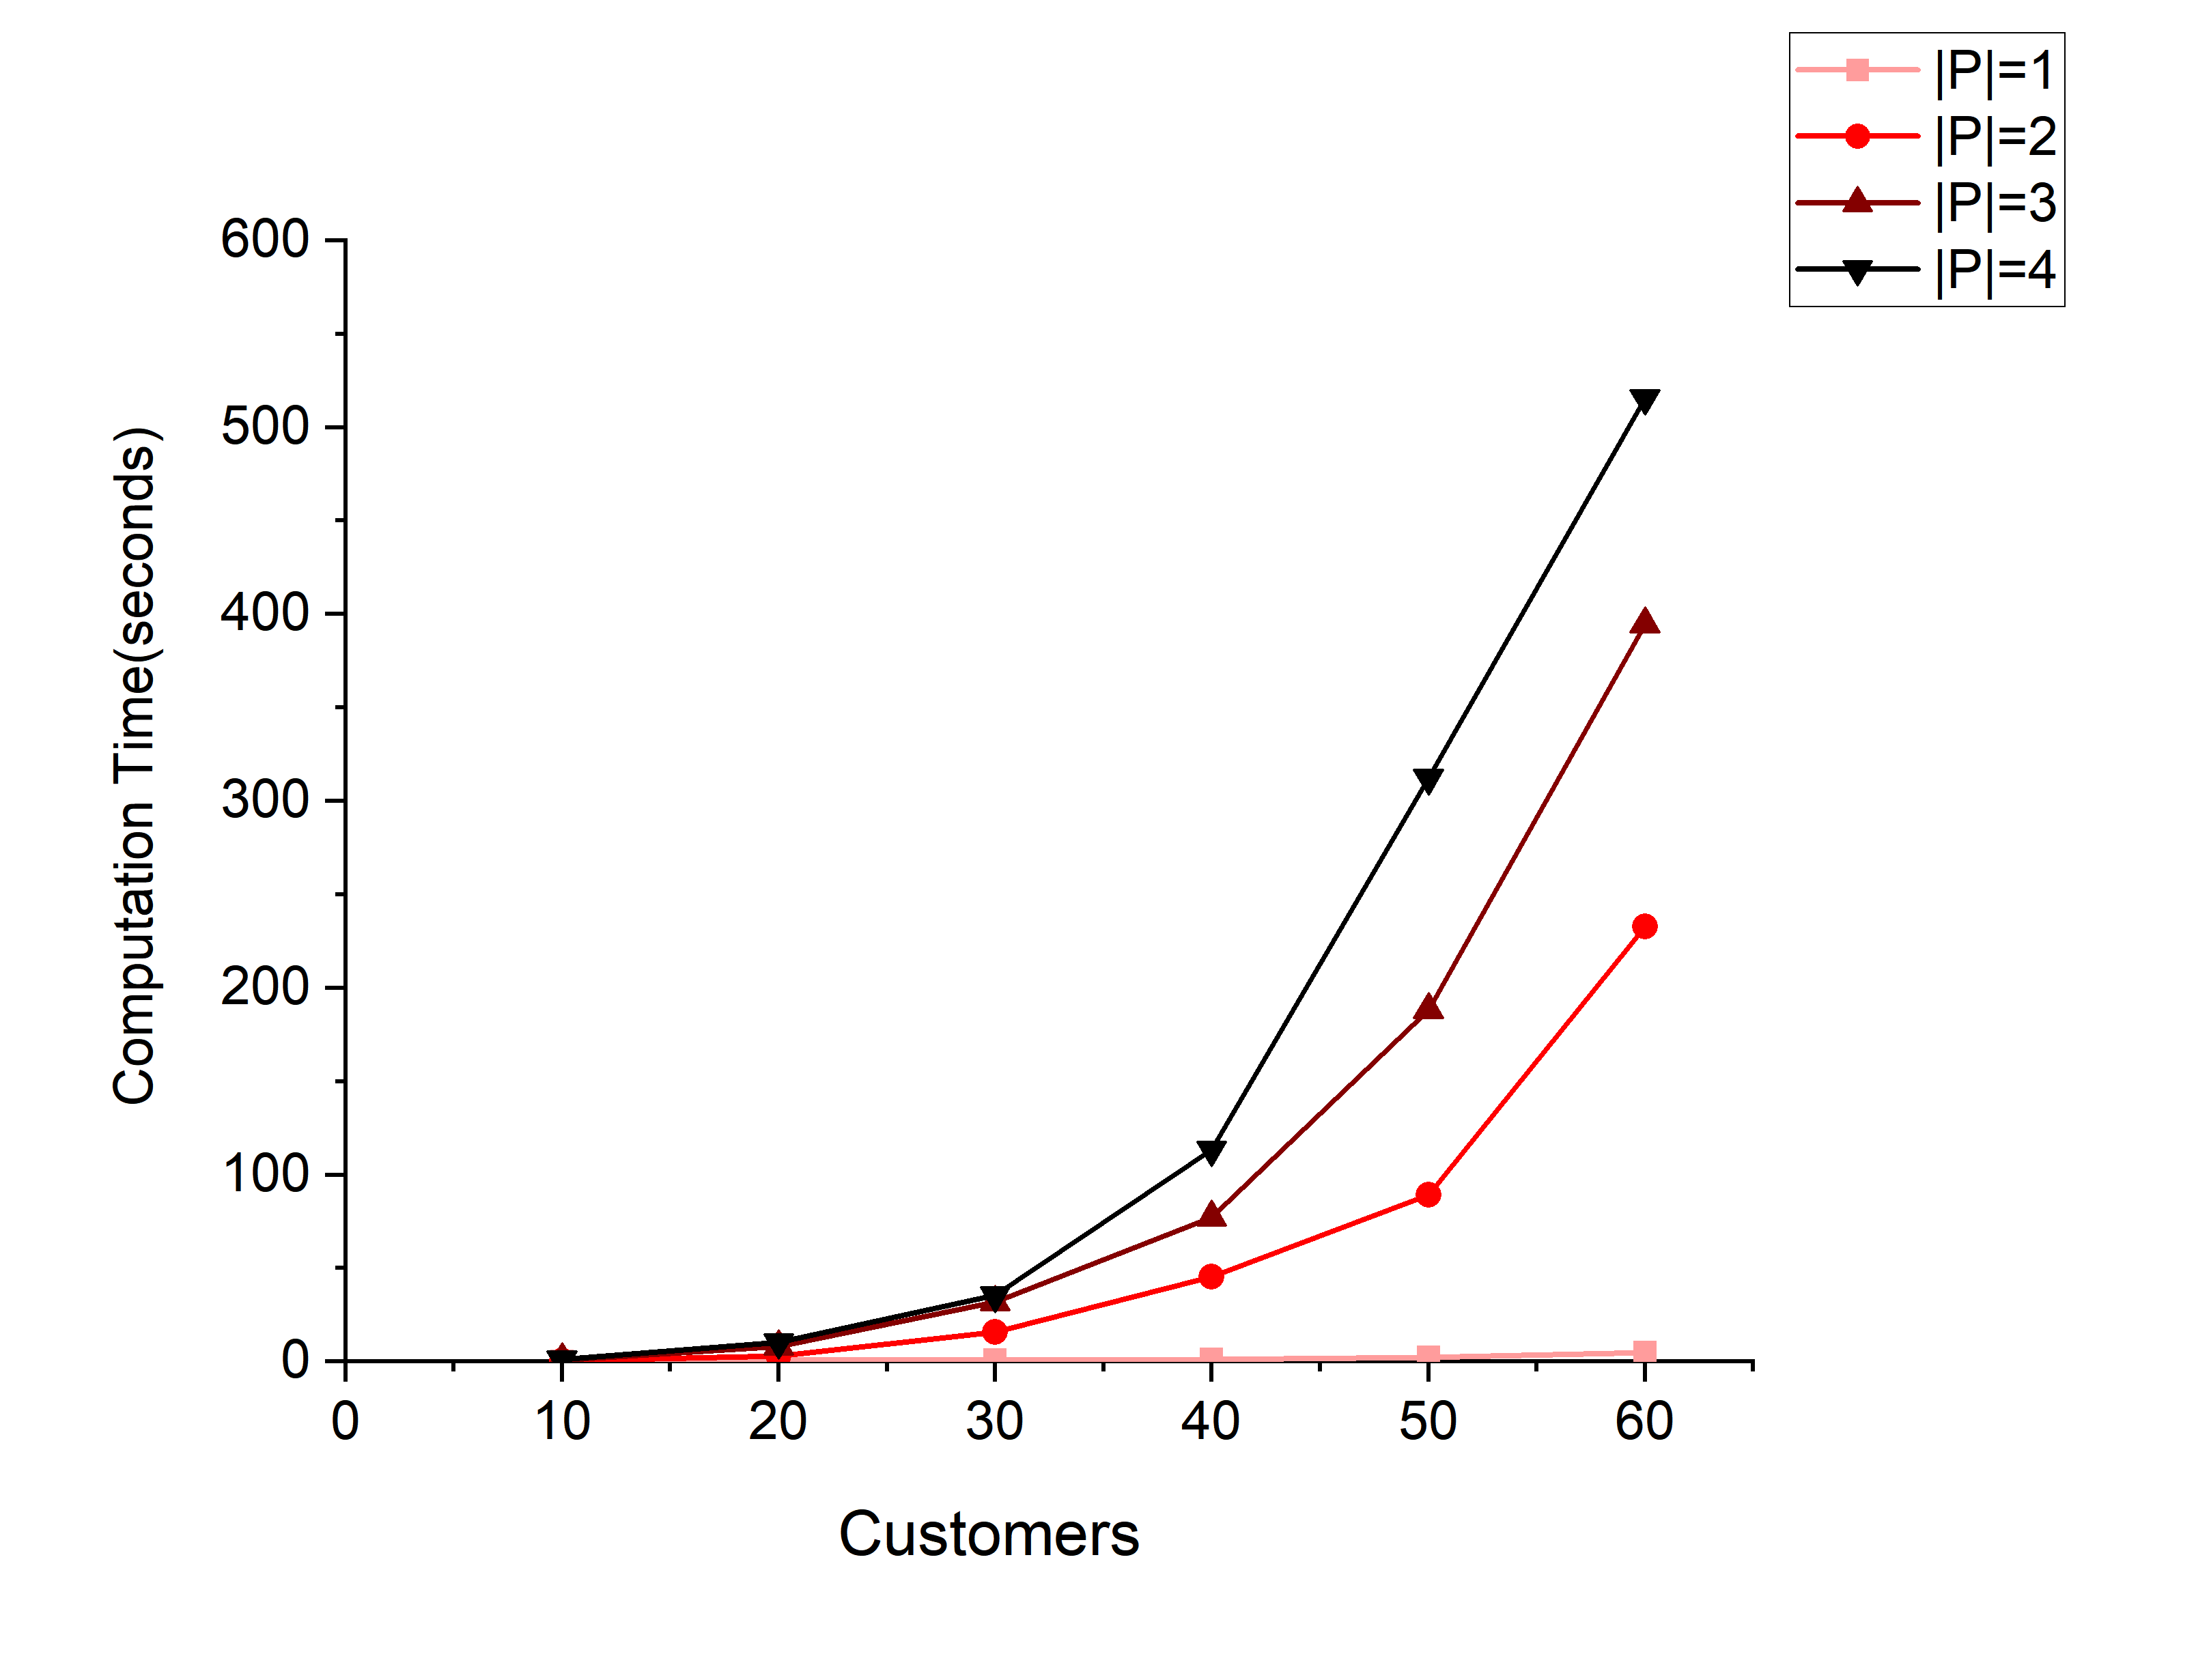
\includegraphics[width=\textwidth]{prod_alns.png}
%       \caption{Number of products}\label{fig:prod_alns}
%     \end{subfigure}
%     \caption{Impact of instance features on average ALNS computation time.}
%     \label{fig:budget}
% \end{figure}

\subsubsection{Impact of the number of the pricing stages}

In this section, we investigate the impacts of the number of the pricing stages on the improvement of the accepted order quantity. As shown in Figure \ref{fig:stagenumber}, the accepted order quantity increases when the number of pricing stages increases. However, the slope of the curve becomes smaller when the number of pricing stages is more than 10. Besides, it is detrimental to the driver experiences if the delivery prices of an order change too frequently. Therefore, to balance the accepted order quantity and the driver experiences, it is reasonable to set the number of pricing stages no more than 10.

\begin{figure}[tb]
    \centering
    \begin{subfigure}[b]{0.2\textwidth}
    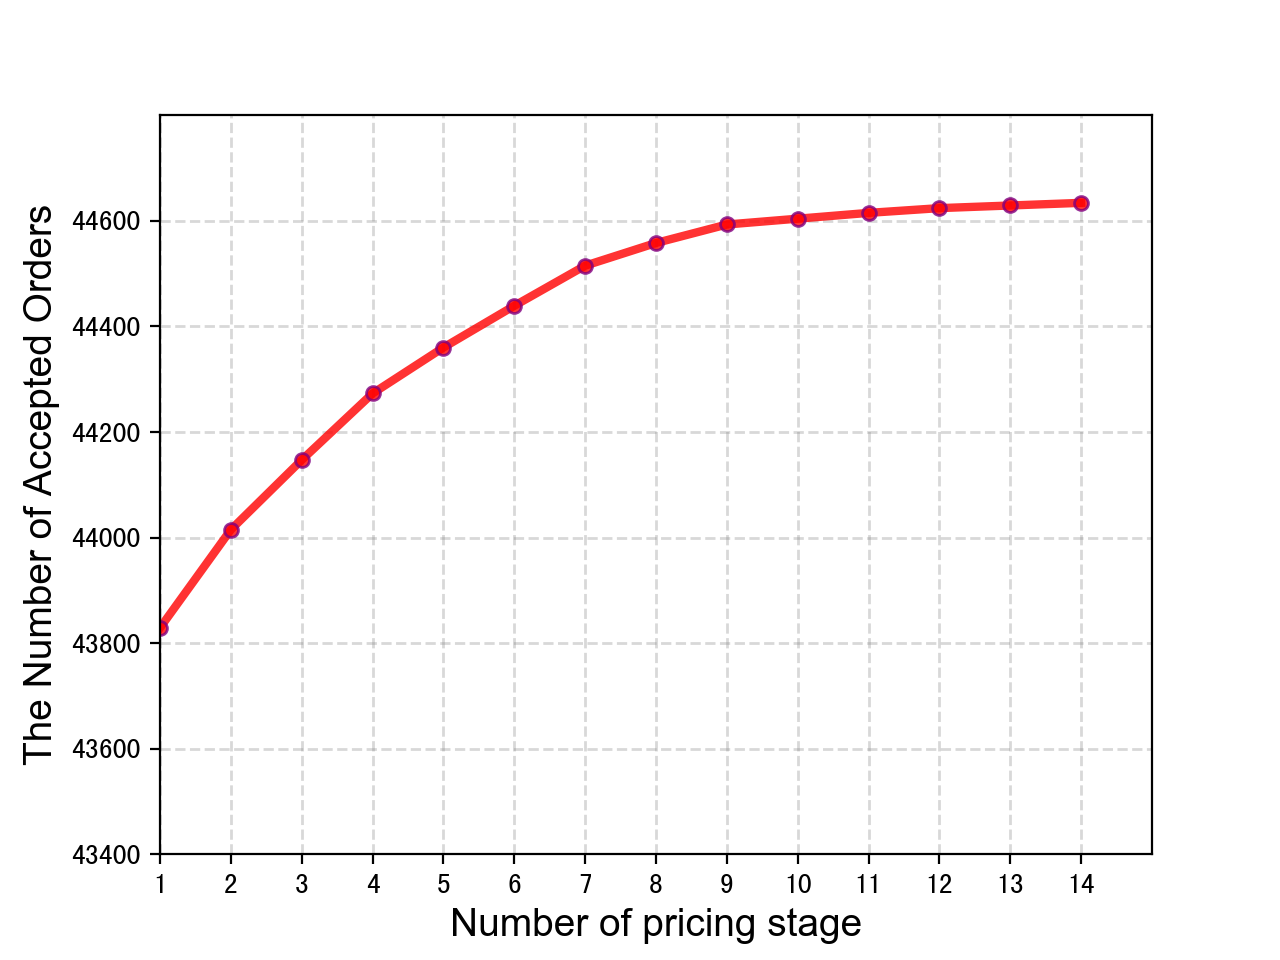
\includegraphics[width=\textwidth]{stagenumber-a.png}
  
        % \caption{Number of vehicles}\label{fig:vehi_alns}
    \end{subfigure}
    \quad
    \begin{subfigure}[b]{0.2\textwidth}
    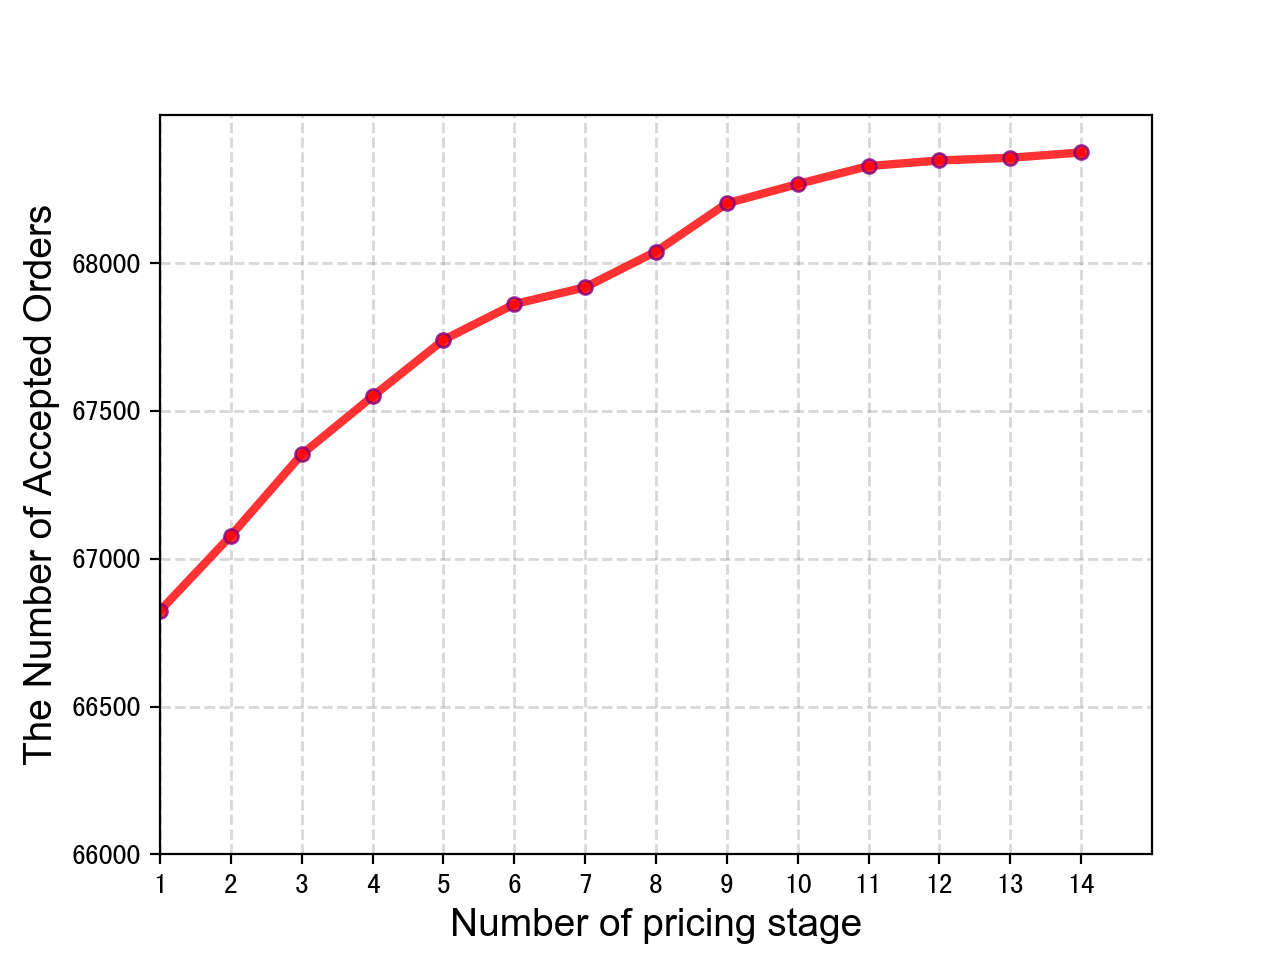
\includegraphics[width=\textwidth]{stagenumber-b.png}
    %  \caption{Number of vehicle compartments}\label{fig:comp_alns}
    \end{subfigure}
    
    \begin{subfigure}[b]{0.2\textwidth}
    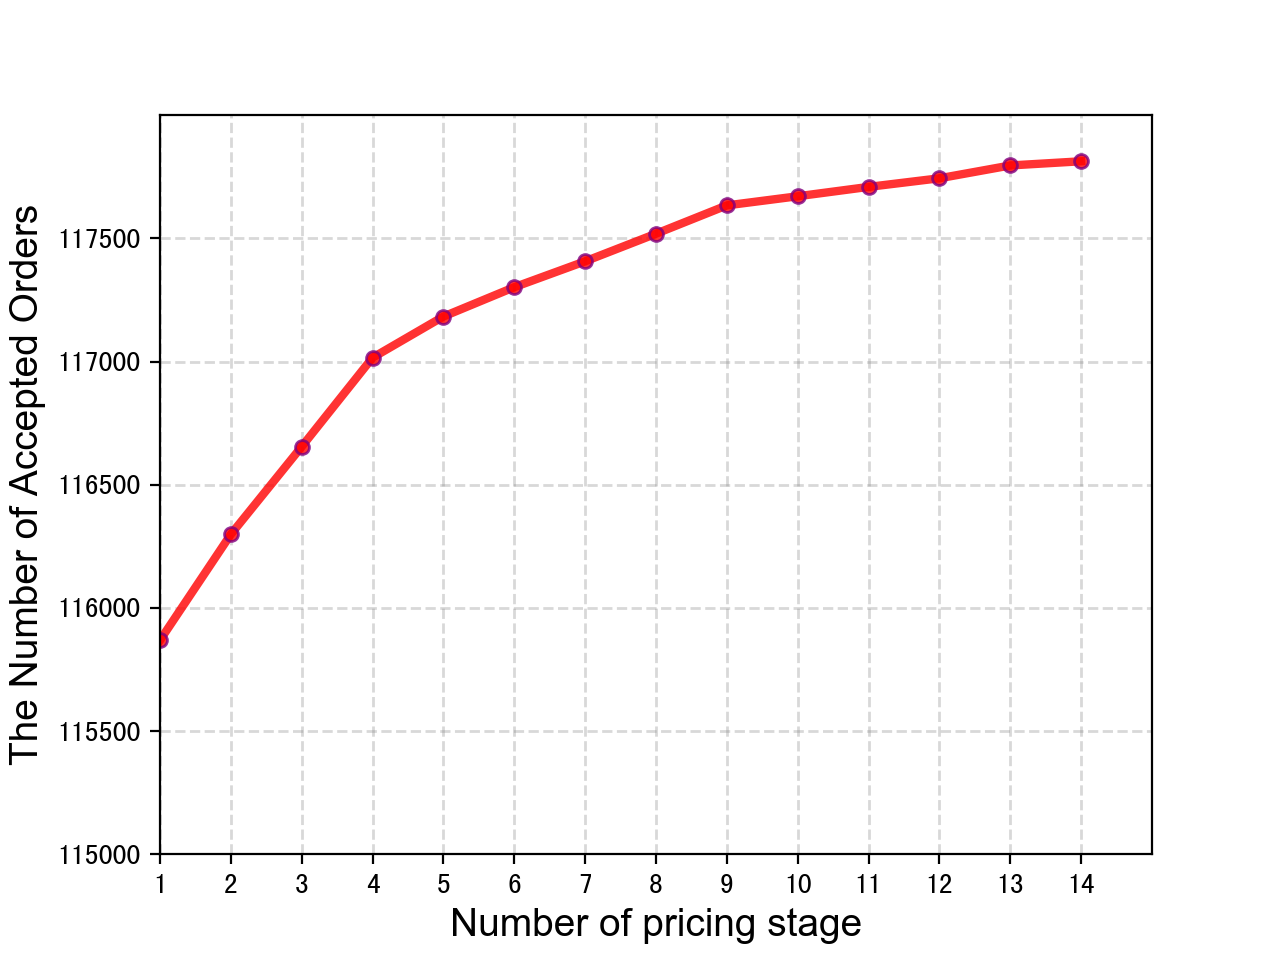
\includegraphics[width=\textwidth]{stagenumber-c.png}
    %   \caption{Compartment capacity}\label{fig:capa_alns}
    \end{subfigure}
    \begin{subfigure}[b]{0.2\textwidth}
    \qquad
    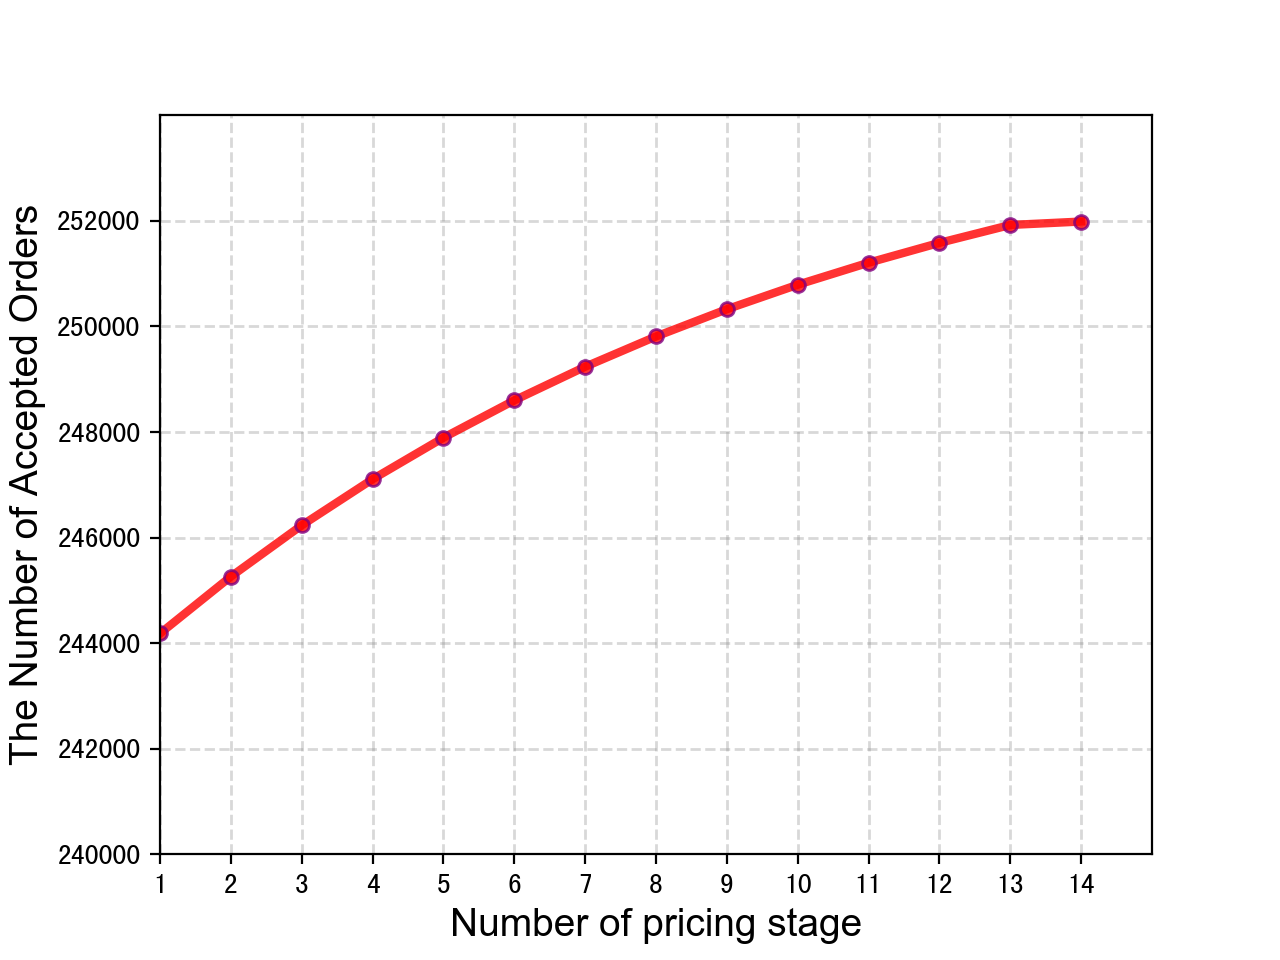
\includegraphics[width=\textwidth]{stagenumber-d.png}
    %   \caption{Number of products}\label{fig:prod_alns}
    \end{subfigure}
     \caption{Impact of the number of the pricing stages on the number of accepted orders.}
    \label{fig:stagenumber}
\end{figure}

\subsubsection{Performance of the multi-stage pricing}

In this section, we analyze the performance of multi-stage pricing method, which is performed using 8 pricing stages with about 6 minutes between two pricing stages. Figure \ref{fig:m-pricing} illustrates the budget allocation on each pricing stage. We observe that the budget allocation on the first(two) stage(s) is negative whereas the other stages are positive. To find out the potential reasons, we investigate the distribution of the accepted order numbers on these pricing stages. As shown in Figure \ref{fig:m-pricing2}, most orders are accepted in the first(two) pricing stage(s) immediately. It means that the accept probability of these orders are relatively high. Recall from Section \ref{sec:pro-model} that our goal is to increase the total accept probabilities of all the orders by relocating part of the delivery price from order A to order B. Therefore, most orders in the first(two) pricing stage(s) play the role of "order A". The budget allocated to the first(two) pricing stage(s) is negative. In other words, the budget is actually saved and accumulated in the first(two) pricing stage(s) and spent on the other pricing stages. The comparison of the results between our method and unified pricing mechanism is presented in Figure \ref{fig:m-pricing2}. As is shown in Figure \ref{fig:m-pricing2}, the accepted orders have a significant increase by using our method. 

\begin{figure}[tb]
    \centering
    \begin{subfigure}[b]{0.2\textwidth}
    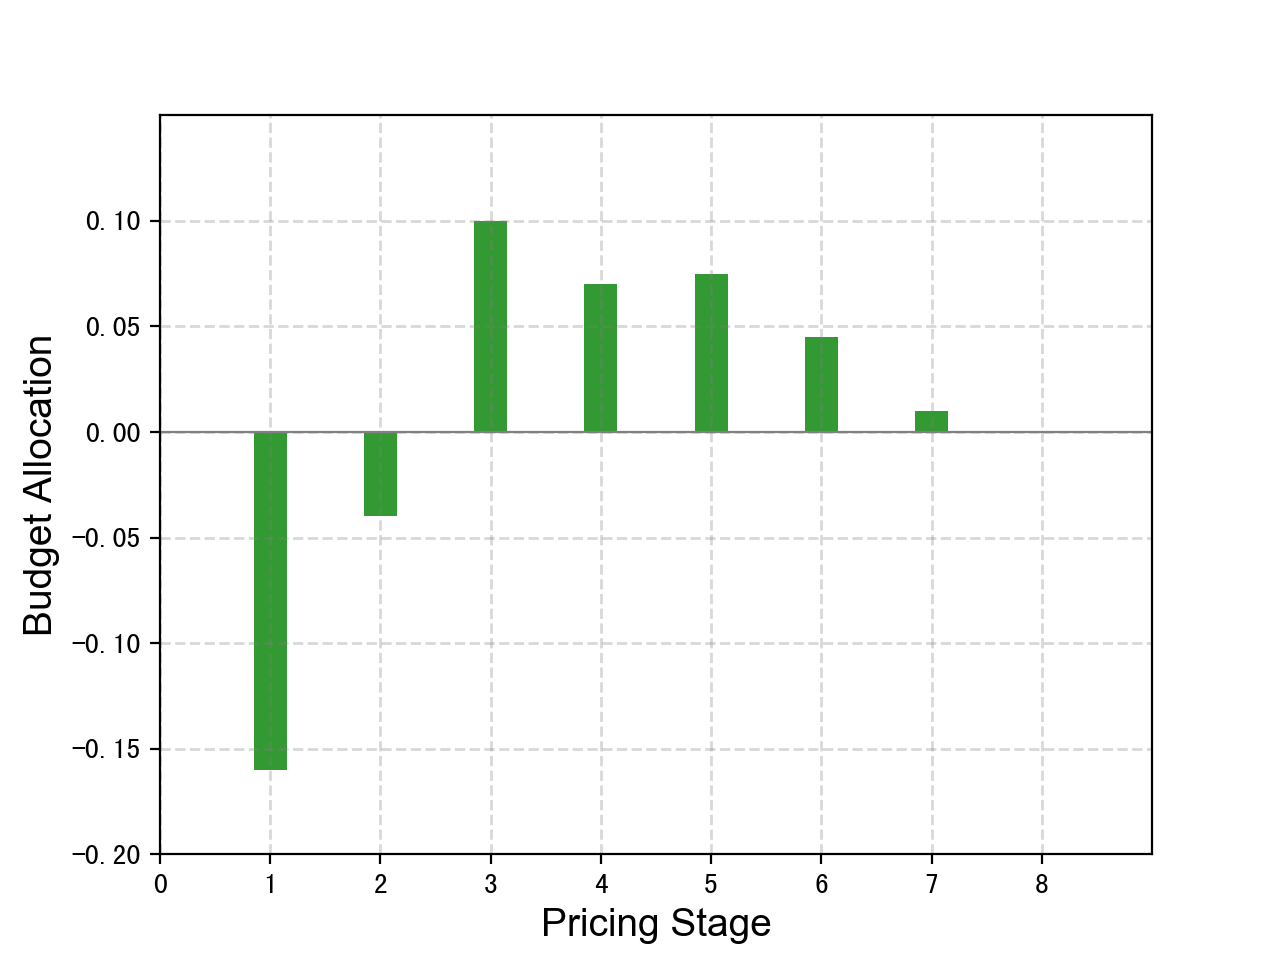
\includegraphics[width=\textwidth]{m-pricing-a.png}
  
        % \caption{Number of vehicles}\label{fig:vehi_alns}
    \end{subfigure}
    \quad
    \begin{subfigure}[b]{0.2\textwidth}
    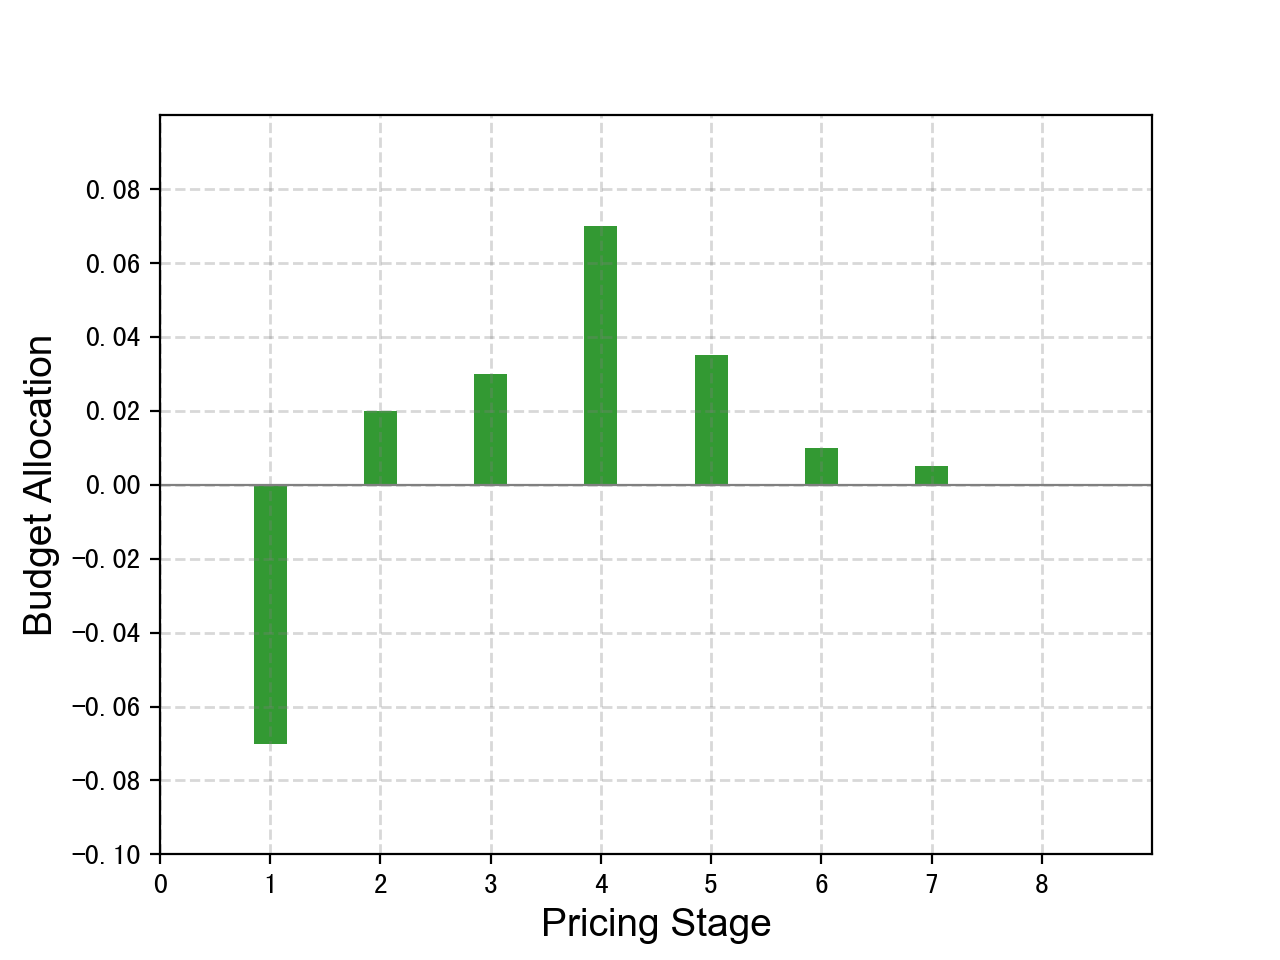
\includegraphics[width=\textwidth]{m-pricing-b.png}
    %  \caption{Number of vehicle compartments}\label{fig:comp_alns}
    \end{subfigure}
    
    \begin{subfigure}[b]{0.2\textwidth}
    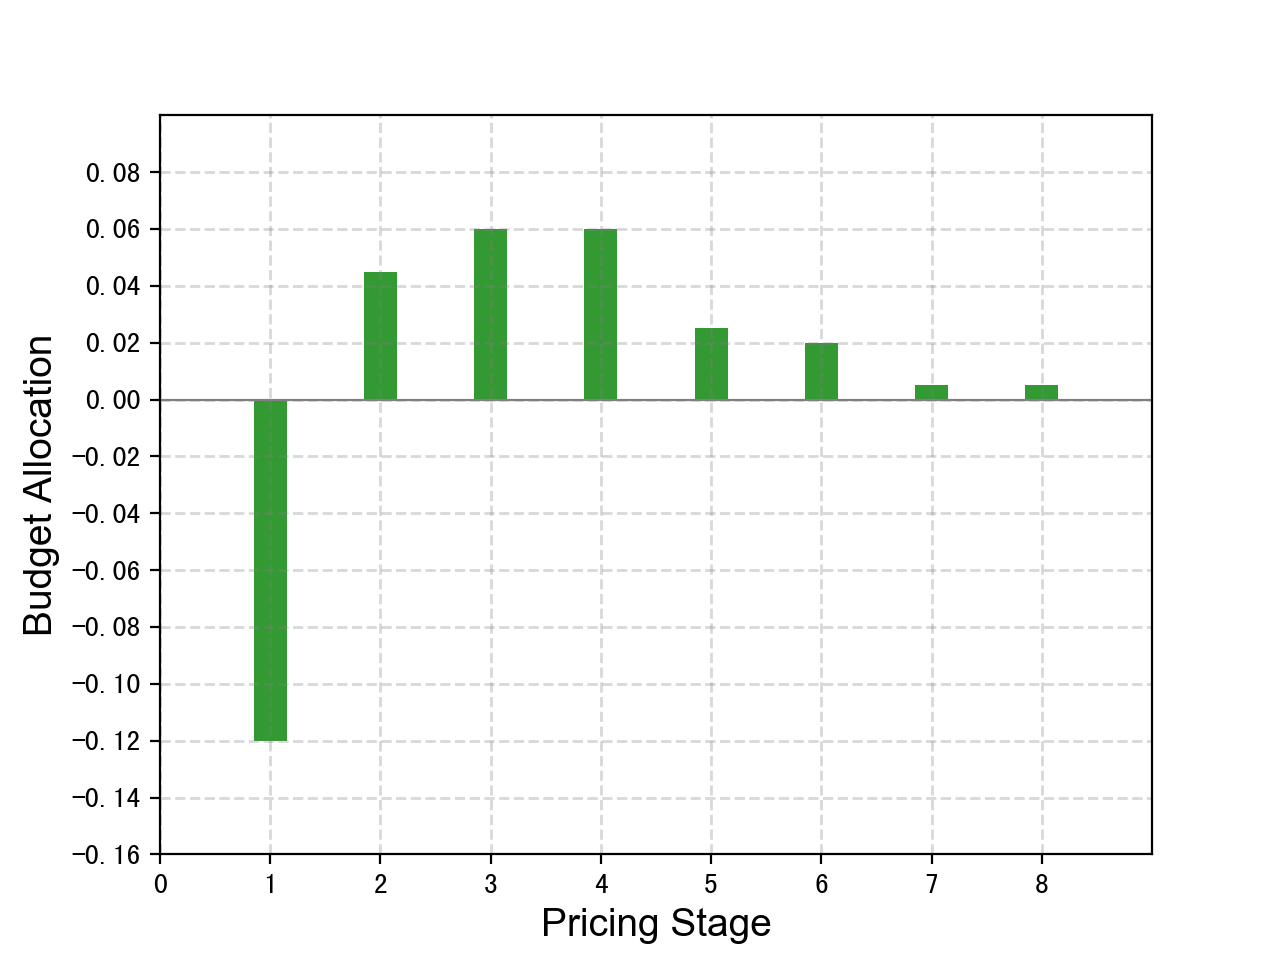
\includegraphics[width=\textwidth]{m-pricing-c.png}
    %   \caption{Compartment capacity}\label{fig:capa_alns}
    \end{subfigure}
    \begin{subfigure}[b]{0.2\textwidth}
    \qquad
    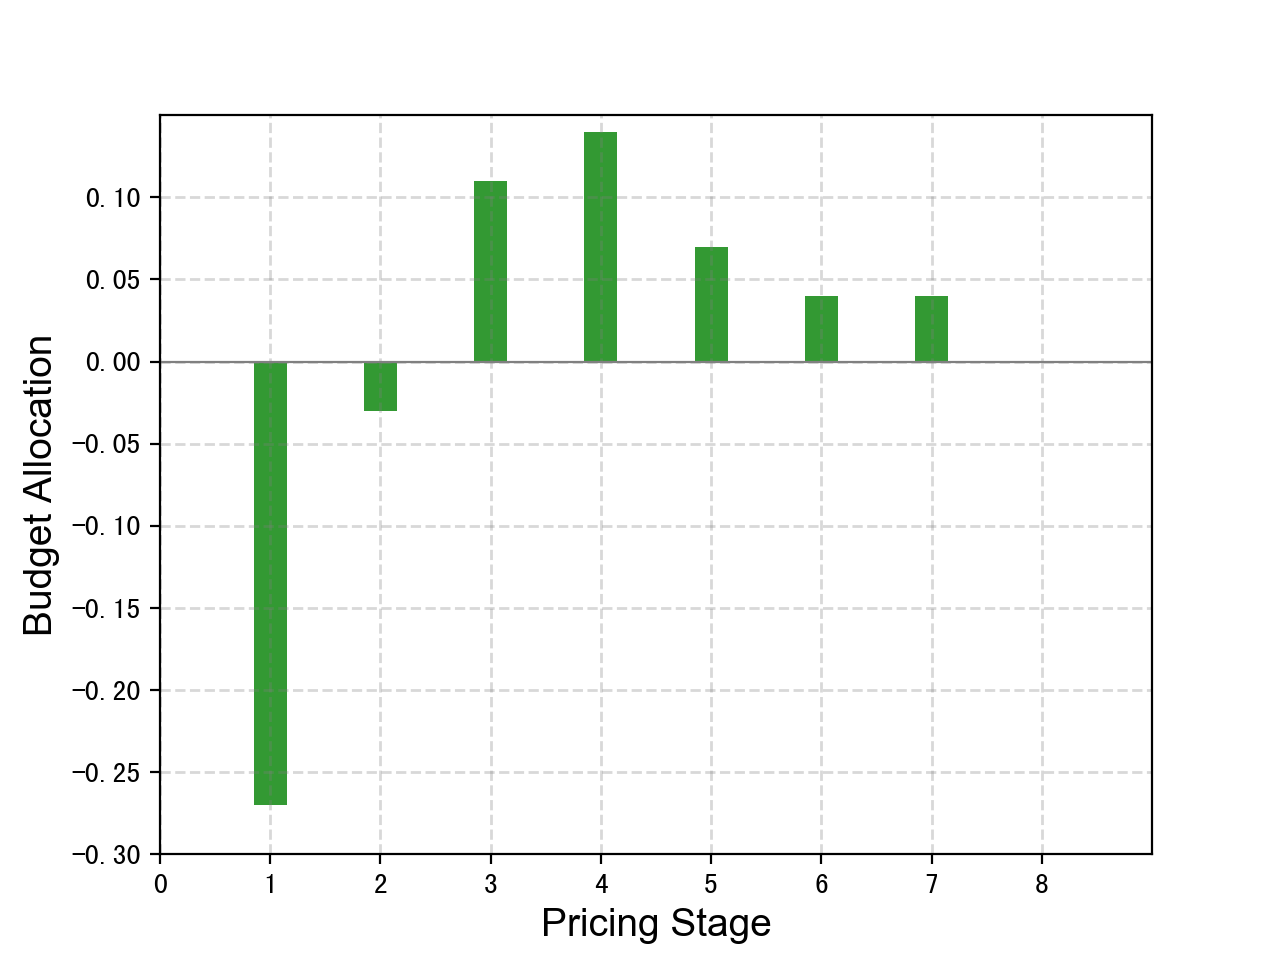
\includegraphics[width=\textwidth]{m-pricing-d.png}
    %   \caption{Number of products}\label{fig:prod_alns}
    \end{subfigure}
    \caption{Budget allocation among all pricing stages.}
    \label{fig:m-pricing}
\end{figure}
\begin{figure}[tb]
    \centering
    \begin{subfigure}[b]{0.2\textwidth}
    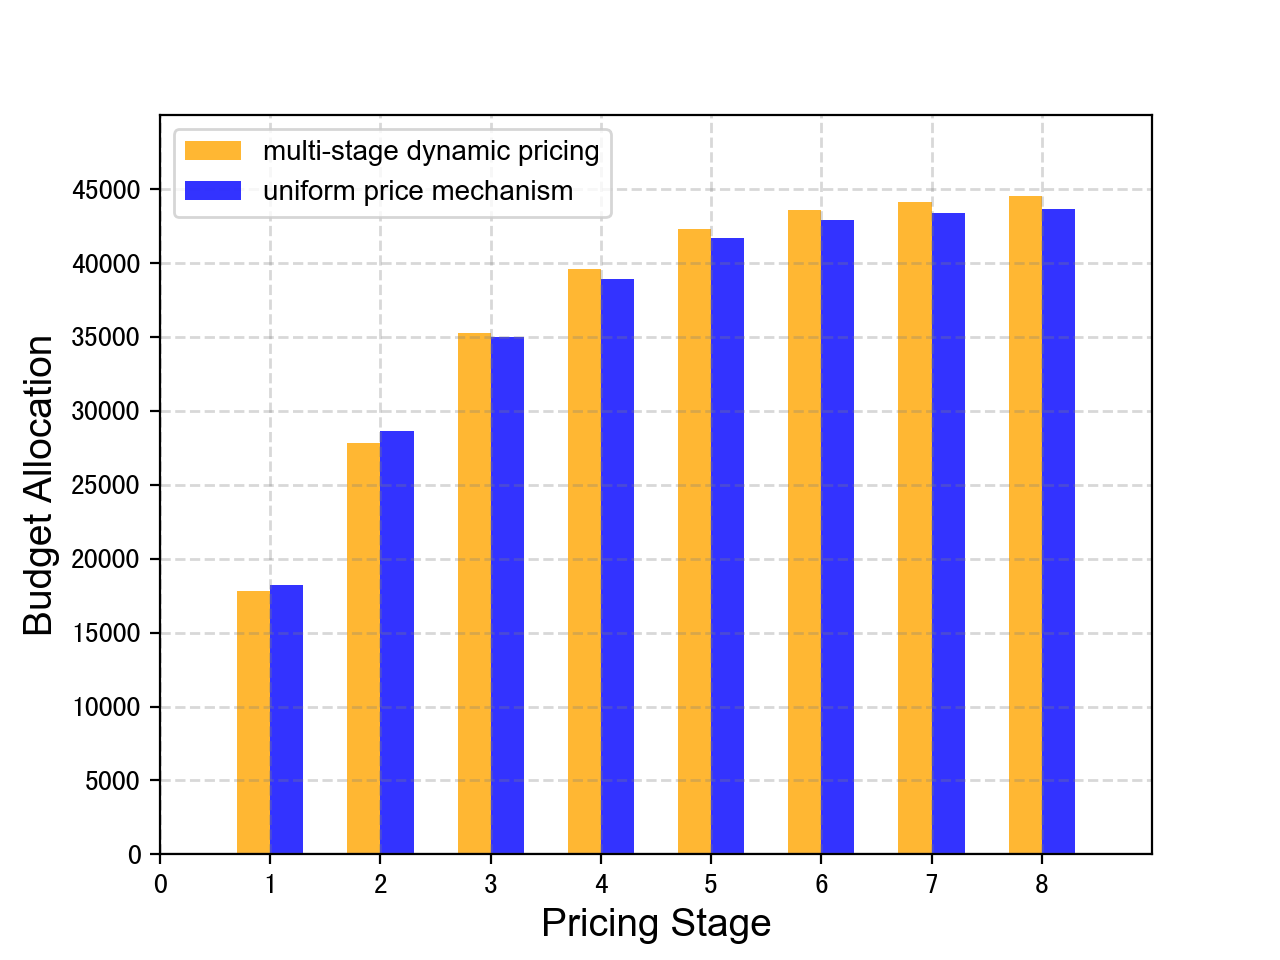
\includegraphics[width=\textwidth]{m-pricing2-a.png}
  
        % \caption{Number of vehicles}\label{fig:vehi_alns}
    \end{subfigure}
    \quad
    \begin{subfigure}[b]{0.2\textwidth}
    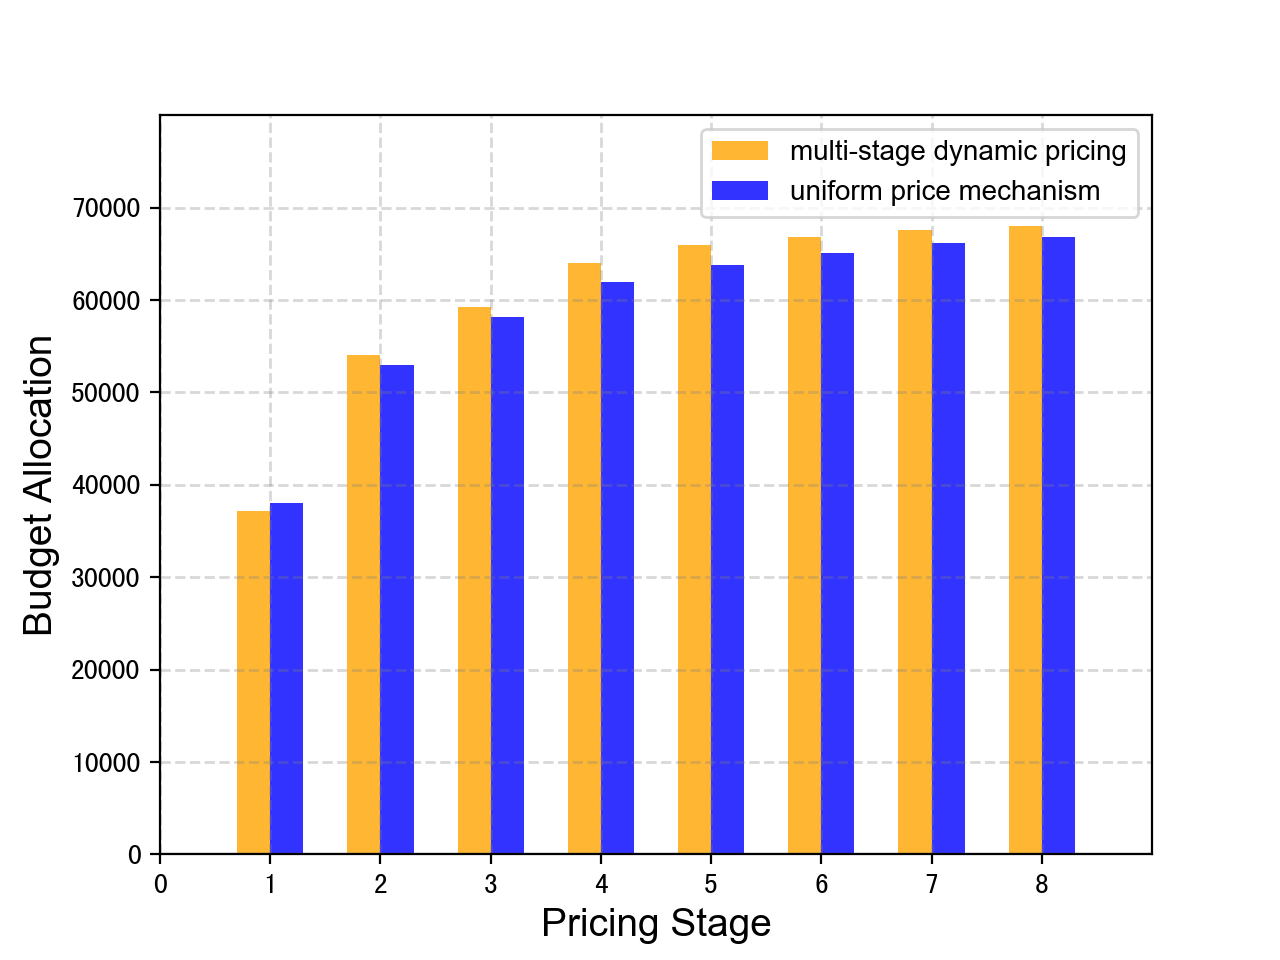
\includegraphics[width=\textwidth]{m-pricing2-b.png}
    %  \caption{Number of vehicle compartments}\label{fig:comp_alns}
    \end{subfigure}
    
    \begin{subfigure}[b]{0.2\textwidth}
    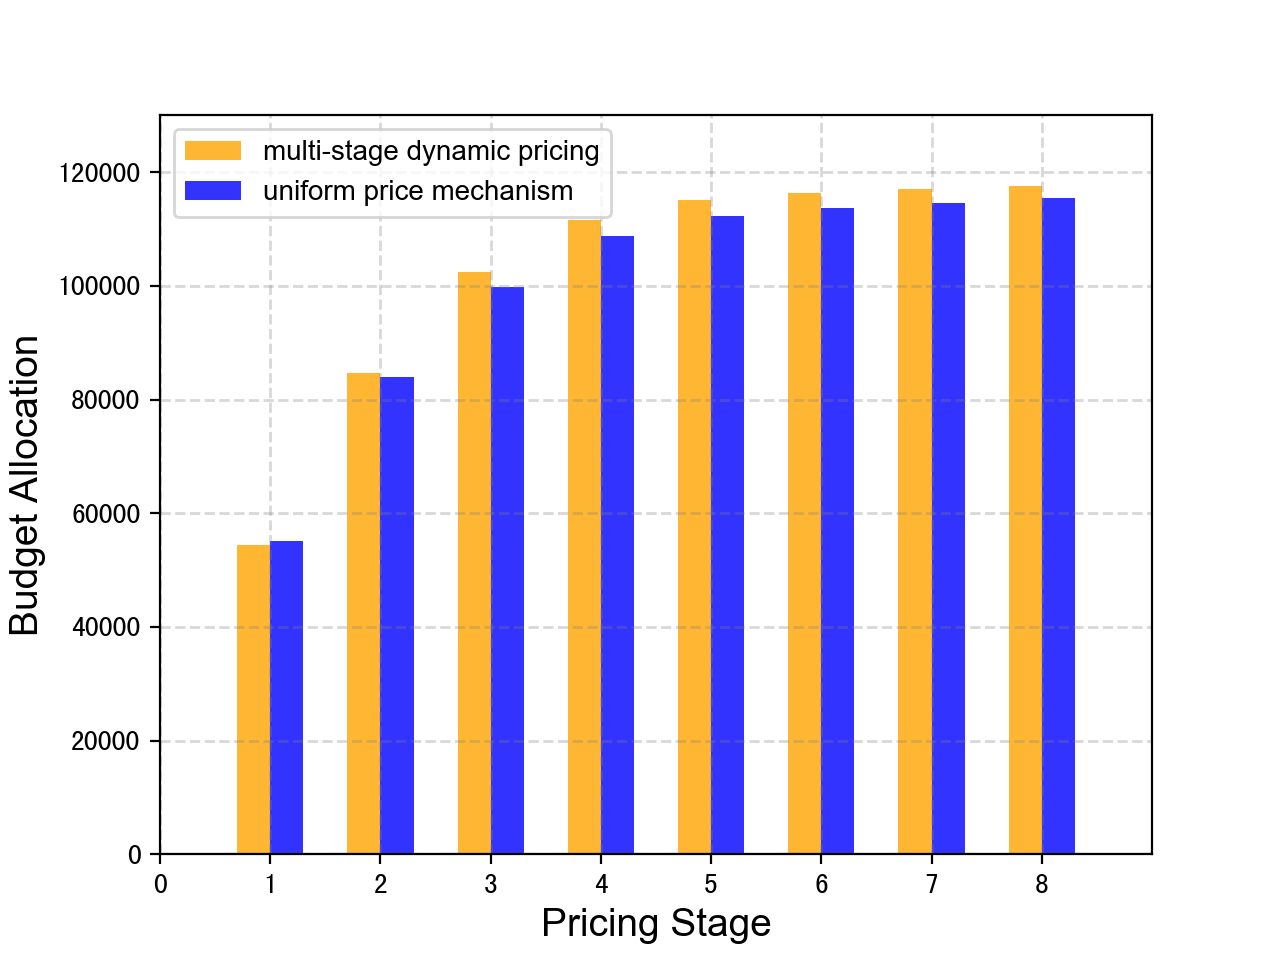
\includegraphics[width=\textwidth]{m-pricing2-c.png}
    %   \caption{Compartment capacity}\label{fig:capa_alns}
    \end{subfigure}
    \begin{subfigure}[b]{0.2\textwidth}
    \qquad
    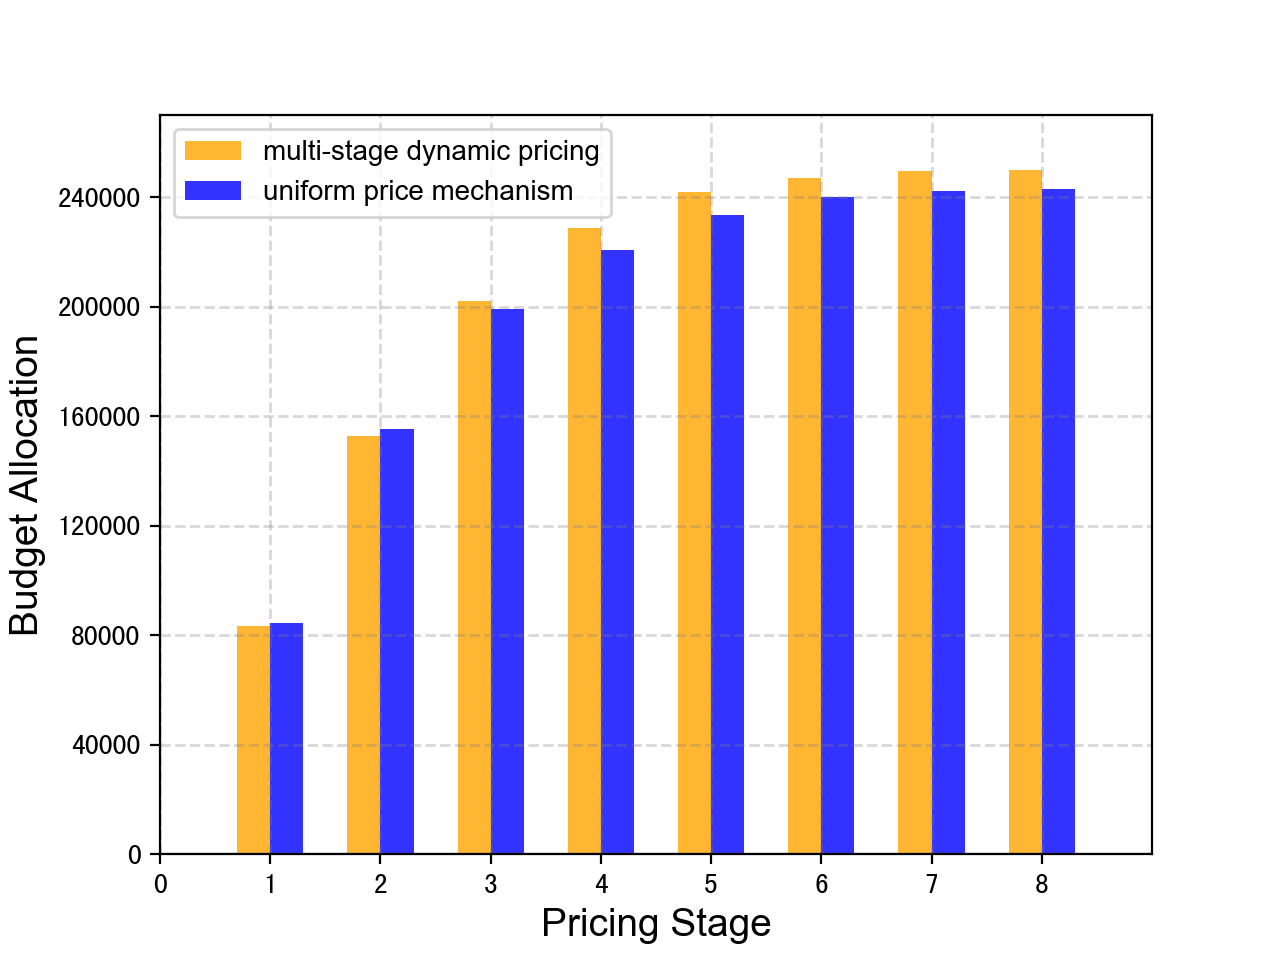
\includegraphics[width=\textwidth]{m-pricing2-d.png}
    %   \caption{Number of products}\label{fig:prod_alns}
    \end{subfigure}
    \caption{The comparison of the number of accepted orders between multi-stage dynamic pricing and uniform pricing mechanism.}
    \label{fig:m-pricing2}
\end{figure}
\subsubsection{Performance of the accept probability model}
As an important part of our framework, the accept probability model is trained and updated daily using the historical data set over the most recent 30 days. In table \ref{tab:eva-model}, we list the performance of different machine learning models for accept probability forecasting. We test these models on the orders all over the country for 30 days. The result shows that DeepFM out perform other models in Area Under the ROC Curve(AUC).
\begin{table}[t]
\caption{Performance of ML Methods on the accept probability model}
\label{tab:eva-model}
\begin{tabular}{l|l}
\toprule
ML method     & AUC   \\
\midrule
GBDT          & 0.743 \\
Random Forest & 0.764 \\
XgBoost       & 0.841 \\
${\rm DeepFM^*}$        & \textbf{0.887}\\
\bottomrule 
\end{tabular}
\end{table}

\subsection{Performance of online A/B tests}
In this section, we introduce our online A/B tests on Meituan meal-delivery platform. 
\subsubsection{Experiment Settings}

We implement our A/B tests on 3 cities in China, which cover 40 areas and 1,740,000 orders are placed per day. The areas in each city are categorized into the experimental group or the control group randomly. We only use our method on the experimental group. The budget on both the experimental group and the control group is posed on 0. To verify the effectiveness of our algorithm, we record the order information data two weeks before and after the start time of the experiment for both experimental group and control group. 

\subsubsection{Implementation of online A/B tests}
The empirical Lagrangian Multiplier for each pricing stage is updated daily and we use an offline algorithm to obtain the parameters by using the historical data set for 30 days before the experiment date. The online algorithm is triggered when an order is presented on the screen of the driver. The pricing stage is inferred through the time from the order placed to the online algorithm triggered. The delivery price of an order is calculated in milliseconds using empirical Lagrangian Multiplier. 

\subsubsection{Results}
Since the order is canceled by the platform if nobody accept it, the most important KPI we concerned is the number of canceled order. As shown in Table \ref{tab:abtest}, the number of canceled order reduced by more than 30\%. The utilization of the budget is another KPI we need to evaluate. Table \ref{tab:abtest} also measures the budget utilization, which is computed as the monthly used budget divided by the given budget at the beginning of a month.  We make best use of the budget without too much budget exceeding with the budget utilization is around 1.0. 


\begin{table}[t]
\caption{Performance of online A/B tests}
\label{tab:abtest}
\begin{tabular}{l|cc}
\toprule
City Name & Canceled Order Reduction & Budget Utilization   \\
\midrule
Nanchang  & 60.82\%             & 0.97 \\
Weihai    & 40.00\%                      &0.93 \\
Zhuhai    & 29.83\%             &1.09\\
\bottomrule
\end{tabular}

\end{table}

\section{Conclusion}\label{sec:conc}
In this paper, we presented a framework of multi-stage dynamic pricing for our meal-delivery platform. Specifically, it helps to adjust the delivery price in time to increase the order accept probabilities. We formally defined the problem and model it by a mathematical programming. A semi-black-box accept probability model was also generated by using a machine learning technique. To solve this problem effectively, we proposed an offline-online algorithm. In offline part, the optimization problem can be solved by dynamic programming and binary search algorithm. The offline results of empirical Lagrangian Multiplier for each stage are used in online part. The computational complexity of online algorithm is O(1) so that it can be solved within milliseconds. Furthermore, this framework is easy to implement, which can be successfully applied to Meituan meal-delivery platform. Both offline experiments and online A/B tests are implemented to verify the effectiveness of our method, which shows the number of canceled order reduced by more than 30\%.

For the future work, we are interested to analyze the approximation error brought by the assumption in Section \ref{sec:alg}. Furthermore, how to solve the problem without the assumption is another topic which is worth exploring. 

%%
%% The acknowledgments section is defined using the "acks" environment
%% (and NOT an unnumbered section). This ensures the proper
%% identification of the section in the article metadata, and the
%% consistent spelling of the heading.


%%
%% The next two lines define the bibliography style to be used, and
%% the bibliography file.
\bibliographystyle{ACM-Reference-Format}
\bibliography{sample-base}

%%
%% If your work has an appendix, this is the place to put it.



\end{document}
\endinput
%%
%% End of file `sample-authordraft.tex'.
